% !TeX spellcheck = hu_HU
% !TeX encoding = UTF-8
% !TeX program = xelatex
\documentclass[11pt,a4paper,oneside]{report}             % Single-side
%\documentclass[11pt,a4paper,twoside,openright]{report}  % Duplex

% thanks to http://tex.stackexchange.com/a/47579/71109
\usepackage{ifxetex}
\usepackage{ifluatex}
\newif\ifxetexorluatex % a new conditional starts as false
\ifnum 0\ifxetex 1\fi\ifluatex 1\fi>0
   \xetexorluatextrue
\fi

\ifxetexorluatex
  \usepackage{fontspec}
\else
  \usepackage[T1]{fontenc}
  \usepackage[utf8]{inputenc}
  \usepackage[lighttt]{lmodern}
\fi

\usepackage[english,magyar]{babel} % Alapértelmezés szerint utoljára definiált nyelv lesz aktív, de később külön beállítjuk az aktív nyelvet.

%\usepackage{cmap}
\usepackage{amsfonts,amsmath,amssymb} % Mathematical symbols.
%\usepackage[ruled,boxed,resetcount,linesnumbered]{algorithm2e} % For pseudocodes. % beware: this is not compatible with LuaLaTeX, see http://tex.stackexchange.com/questions/34814/lualatex-and-algorithm2e
\usepackage{booktabs} % For publication quality tables for LaTeX
\usepackage{graphicx}

\usepackage{jslistings}
%\usepackage{fancyhdr}
%\usepackage{lastpage}

\usepackage{anysize}
%\usepackage{sectsty}
\usepackage{setspace} % For setting line spacing

\usepackage[unicode]{hyperref} % For hyperlinks in the generated document.
\usepackage{xcolor}
\usepackage{listings} % For source code snippets.

\usepackage[amsmath,thmmarks]{ntheorem} % Theorem-like environments.

\usepackage[hang]{caption}

\singlespacing

\newcommand{\selecthungarian}{
	\selectlanguage{magyar}
	\setlength{\parindent}{2em}
	\setlength{\parskip}{0em}
	\frenchspacing
}

\newcommand{\selectenglish}{
	\selectlanguage{english}
	\setlength{\parindent}{0em}
	\setlength{\parskip}{0.5em}
	\nonfrenchspacing
	\renewcommand{\figureautorefname}{Figure}
	\renewcommand{\tableautorefname}{Table}
	\renewcommand{\partautorefname}{Part}
	\renewcommand{\chapterautorefname}{Chapter}
	\renewcommand{\sectionautorefname}{Section}
	\renewcommand{\subsectionautorefname}{Section}
	\renewcommand{\subsubsectionautorefname}{Section}
}

\usepackage[numbers]{natbib}
\usepackage{xspace}


%TODO Set the main variables
\newcommand{\vikszerzoVezeteknev}{Király}
\newcommand{\vikszerzoKeresztnev}{Bálint Martin}

\newcommand{\vikkonzulensAMegszolitas}{}
\newcommand{\vikkonzulensAVezeteknev}{Schulcz}
\newcommand{\vikkonzulensAKeresztnev}{Róbert}

\newcommand{\vikkonzulensBMegszolitas}{}
\newcommand{\vikkonzulensBVezeteknev}{}
\newcommand{\vikkonzulensBKeresztnev}{}

\newcommand{\vikkonzulensCMegszolitas}{}
\newcommand{\vikkonzulensCVezeteknev}{}
\newcommand{\vikkonzulensCKeresztnev}{}

\newcommand{\vikcim}{Leltározási feladatokat segítő, grafikus felülettel rendelkező adatbázis tervezése és fejlesztése} % Cím
\newcommand{\viktanszek}{\bmehit} % Tanszék
\newcommand{\vikdoktipus}{\bsc} % Dokumentum típusa (\bsc vagy \msc)
\newcommand{\vikmunkatipusat}{szakdolgozatot} % a "hallgató nyilatkozat" részhez: szakdolgozatot vagy diplomatervet

\input{include/tdk-variables}
\newcommand{\szerzoMeta}{\vikszerzoVezeteknev{} \vikszerzoKeresztnev} % egy szerző esetén

%--------------------------------------------------------------------------------------
% Elnevezések
%--------------------------------------------------------------------------------------
\newcommand{\bme}{Budapesti Műszaki és Gazdaságtudományi Egyetem}
\newcommand{\vik}{Villamosmérnöki és Informatikai Kar}

\newcommand{\bmehit}{Hálózati Rendszerek és Szolgáltatások Tanszék}

\newcommand{\keszitette}{Készítette}
\newcommand{\konzulens}{Konzulens}

\newcommand{\bsc}{Szakdolgozat}
\newcommand{\msc}{Diplomaterv}
\newcommand{\tdk}{TDK dolgozat}
\newcommand{\bsconlab}{BSc Önálló laboratórium}
\newcommand{\msconlabi}{MSc Önálló laboratórium 1.}
\newcommand{\msconlabii}{MSc Önálló laboratórium 2.}

\newcommand{\pelda}{Példa}
\newcommand{\definicio}{Definíció}
\newcommand{\tetel}{Tétel}

\newcommand{\bevezetes}{Bevezetés}
\newcommand{\koszonetnyilvanitas}{Köszönetnyilvánítás}
\newcommand{\fuggelek}{Függelék}

% Opcionálisan átnevezhető címek
%\addto\captionsmagyar{%
%\renewcommand{\listfigurename}{Saját ábrajegyzék cím}
%\renewcommand{\listtablename}{Saját táblázatjegyzék cím}
%\renewcommand{\bibname}{Saját irodalomjegyzék név}
%}

\newcommand{\szerzo}{\vikszerzoVezeteknev{} \vikszerzoKeresztnev}
\newcommand{\vikkonzulensA}{\vikkonzulensAMegszolitas\vikkonzulensAVezeteknev{} \vikkonzulensAKeresztnev}
\newcommand{\vikkonzulensB}{\vikkonzulensBMegszolitas\vikkonzulensBVezeteknev{} \vikkonzulensBKeresztnev}
\newcommand{\vikkonzulensC}{\vikkonzulensCMegszolitas\vikkonzulensCVezeteknev{} \vikkonzulensCKeresztnev}

\newcommand{\selectthesislanguage}{\selecthungarian}

\bibliographystyle{huplain}

\def\lstlistingname{lista}

\newcommand{\appendixnumber}{6}  % a fofejezet-szamlalo az angol ABC 6. betuje (F) lesz


\input{include/preamble}
\renewcommand{\lstlistingname}{kódrészlet}

%--------------------------------------------------------------------------------------
% Table of contents and the main text
%--------------------------------------------------------------------------------------
\begin{document}

\pagenumbering{gobble}
\nocite{*}


\selectthesislanguage


\makeatletter

\renewcommand*{\ext@figure}{lot}

\let\c@figure\c@table

\let\ftype@figure\ftype@table

\let\listoftableandfigures\listoftables

\renewcommand*\listtablename{List of Tables and figures}

\makeatother

%TODO Titlepage
%~~~~~~~~~~~~~~~~~~~~~~~~~~~~~~~~~~~~~~~~~~~~~~~~~~~~~~~~~~~~~~~~~~~~~~~~~~~~~~~~~~~~~~
\include{include/titlepage}		   % Szakdolgozat/Diplomaterv címlap

% Table of Contents
%~~~~~~~~~~~~~~~~~~~~~~~~~~~~~~~~~~~~~~~~~~~~~~~~~~~~~~~~~~~~~~~~~~~~~~~~~~~~~~~~~~~~~~
\tableofcontents\vfill


% Declaration and Abstract
%~~~~~~~~~~~~~~~~~~~~~~~~~~~~~~~~~~~~~~~~~~~~~~~~~~~~~~~~~~~~~~~~~~~~~~~~~~~~~~~~~~~~~~
\include{include/declaration} %TODO Hallgatói nyilatkozat -- TDK és OTDK esetén törlendő!
% !TeX spellcheck = hu_HU
\pagenumbering{roman}
\setcounter{page}{1}

\selecthungarian

%----------------------------------------------------------------------------
% Abstract in Hungarian
%----------------------------------------------------------------------------
\chapter*{Kivonat}\addcontentsline{toc}{chapter}{Kivonat}

Rengeteg raktárkezelő alkalmazás érhető el a piacon, azonban a térképes nézet egy ritka funkciónak számít ezekben a rendszerekben. Az erre alkalmas szoftverek rendszerint előredefiniált térképpel dolgoznak.

A szakdolgozatom célja egy olyan raktár kezelő rendszer tervezése és fejlesztése, amely lehetővé teszi az eszközök pozíciójának pontos meghatározását a raktáron belül, mindezt dinamikusan. A rendszer segítségével a felhasználók képesek a raktár méretét és elrendezését is meghatározni, így a pontos igényeknek megfelelő alkalmazást kaphatnak.

A feladat megvalósítása során kutatást végeztem a meglévő rendszerekről, majd elkészítettem a feladat specifikációt, valamint az alkalmazás wireframe-eit. Ezek definiálása után elkezdtem az architekturális tervezést, majd neki láttam az alkalmazás implementálásának. Az üzleti logikát és a kliens oldali megjelenítést is JavaScript, pontosabban annak egy superset-jével, a TypeScript-tel valósítottam meg. A fejlesztés után és közben teszteket készítettem a működés ellenőrzése érdekében.

\vfill
\selectenglish

%----------------------------------------------------------------------------
% Abstract in English
%----------------------------------------------------------------------------
\chapter*{Abstract}\addcontentsline{toc}{chapter}{Abstract}

There is a great deal of warehouse management applications available in the market, however, the map view is a rare feature in these systems. The warehouse management software usually works with a predefined maps.

The aim of my dissertation is to design and develop a warehouse management system that allows to determine the exact position of items within the warehouse. With the help of the system, users can also set the size and layout of the warehouse, so they can get the application that suits their exact needs.

During the implementation of the task, I conducted research on the existing systems and then prepared the task specification as well as the application wireframes. After defining these, I started architectural design and after that I started to work on the implementation of the application. I also implemented the business logic and the client-side visualization with JavaScript, more precisely with its superset, TypeScript. After and during the development, I did tests to validate the operation.

\vfill
\selectthesislanguage

\newcounter{romanPage}
\setcounter{romanPage}{\value{page}}
\stepcounter{romanPage}    %TODO Összefoglaló -- TDK és OTDK esetén nem kötelező


% The main part of the thesis
%~~~~~~~~~~~~~~~~~~~~~~~~~~~~~~~~~~~~~~~~~~~~~~~~~~~~~~~~~~~~~~~~~~~~~~~~~~~~~~~~~~~~~~
\pagenumbering{arabic}

%TODO import your own content
% !TeX spellcheck = hu_HU
%----------------------------------------------------------------------------
\chapter{\bevezetes}
%----------------------------------------------------------------------------

A félév során a feladatom egy olyan grafikus felülettel ellátott leltár rendszer tervezése és fejlesztése volt, melynek segítségével az alapvető leltári funkciókon felül könnyedén behatárolhatjuk a leltárba vett eszközök pontos helyzetét a raktárunkon belül egy grafikus “térkép” segítségével.

A dolgozatom során első körben egy részletes specifikációt készítettem, melyben taglaltam az alkalmazással szemben támasztott funkcionális és nem-funkcionális követelményeket.
Ezután megterveztem a webalkalmazás felhasználói felületét, egyszerű wireframe-ek segítségével.

A specifikáció és a wireframe-ek elkészítése után kiválasztottam a használni kívánt technológiákat és megterveztem az alkalmazás architekturális felépítését.

Az alkalmazás két fő részből áll, frontend és backend. Utóbbi tartalmazza az üzleti logikát és az adatbázis kommunikációt, míg a frontend az adatok lekéréséért és megjelenítéséért felel, valamint a felhasználói interakciók által eljuttatja a módosításokat a backend részére.
Ezek fejlesztését párhuzamosan végeztem. Minden egyes funkciónak először elkészítettem a backend oldali implementációját, majd hozzáláttam a frontend oldali kód fejlesztésének. Sok esetben szükséges volt a backend módosításra a frontend fejlesztése közben is.

Az alkalmazás tervezésén és fejlesztésén kívül az üzemeltetés előkészítését is elvégeztem, valamint bevezettem olyan megoldásokat, melyek a fejlesztés minőségét segítették elő.

Végül a tesztelésre fektettem a hangsúlyt, amely közben a felmerülő hibák javítását eszközöltem az alkalmazásban.

A dolgozat fejezeteivel próbáltam ezt a sorrendet tartani, hogy az olvasó számára is könnyen követhető legyen a folyamat és az összefüggések.
%----------------------------------------------------------------------------
\chapter{Feladat specifikáció}
%----------------------------------------------------------------------------

A fejezet kitér az alkalmazással szemben támasztott funkcionális és nem funkcionális követelményekre.

%----------------------------------------------------------------------------
\section{Funkciónális követelmények}
%----------------------------------------------------------------------------

%----------------------------------------------------------------------------
\subsection{Regisztráció}
%----------------------------------------------------------------------------
Az elkészítendő alkalmazásban legyen lehetőség felhasználót létrehozni egy regisztrációs oldalon.
A regisztráció során a felhasználó nevét, email címét, jelszavát valamint a jelszavának megerősítését kérjük.
További fontos követelmény, hogy egy email címhez csak egy felhasználó tartozhat

%----------------------------------------------------------------------------
\subsection{Bejelentkezés}
%----------------------------------------------------------------------------
A regisztráció során megadott email cím és jelszó segítségével a látogatónak képesnek kell lennie authentikálni magát.
A rendszer csak authentikált felhasználók számára legyen elérhető.
Nem authentikált felhasználóknak csak a bejelentkezés és a regisztráció opciókat kínáljuk fel.

%----------------------------------------------------------------------------
\subsection{Raktár épületek kezelése}
%----------------------------------------------------------------------------
Az alkalmazással szemben követelmény, hogy képesnek kell lennie több raktár (raktár épület) kezelését.
Ez alatt értjük a raktár létrehozását, és szerkesztését valamint az ezekhez tartozó jogosultságok menedzselését.
A raktárról tároljuk a méreteit, a nevét és természetesen a szerkesztésre jogosult felhasználók listáját.

%----------------------------------------------------------------------------
\subsection{Tárolók kezelése}
%----------------------------------------------------------------------------
Minden raktárba tárolók helyezhetőek. A tárolókat a nevükkel és meretükkel egyűtt rögzíthetjuk.
Amennyiben a felhasználó rendelkezik a megfelelő jogosultsággal az adott raktáron belül, legyen lehetősége a tárolók szerkesztésre, létrehozására és törlésére.

%----------------------------------------------------------------------------
\subsection{Eszközök kezelése}
%----------------------------------------------------------------------------
A hierarchia harmadik szintjén helyezkednek el az eszközökök. 
Minden eszköz rendelkezzen az alábbi tulajdonságokkal.
Név, amely az egyszerű azonosítást és a kereshetőséget biztosítja.
Érték, ami az eszköz raktárba vételekori értékét tartalmazza.
Minden egyes leltárba vett eszköhöz legyen lehetőségünk a kiadások felvételére.
Minden kiadáshoz egy összeg és egy leírás tartozik, amely a kiadás okának magyarázatára szolgál.

%----------------------------------------------------------------------------
\subsection{Raktár térképes nézettel}
%----------------------------------------------------------------------------
A raktárakban a tárolók elhelyezkedését jelenítsük meg egy felülnézeti, térképes nézet formájában is.
A tárolók mozgatását nem szükséges megvalósítani ezen a térképen.
Ennek oka, hogy míg az eszközök poziciója gyakran változik a tárolók fixen telepítve vannak.
Ennek a funkciónak a nem implementálása felesleges félreértések elkerülését is szolgálja.

%----------------------------------------------------------------------------
\subsection{Tároló térképes nézettel}
%----------------------------------------------------------------------------
Minden tároló oldalán jelenítsünk meg egy képet a tároló tartalmával.
A tárolt eszközöket egyszerű téglalappal reprezentáljuk.
Fontos követelmény, hogy a ezen a nézeten legyen lehetőség az eszközök mozgatására is.
A mozgatást a felhasználó a mozgatni kívánt elemre kattintva, majd az egér ball billentyűjét lenyomva mozgathatja a tárolón belül.
A fent leírt módszer segítségével legyen lehetőség egy ideiglenes tárolóba rakni. 
Ezt az ideiglenes tárolót jelenítsük meg minden (az adott raktárban lévő) tároló oldalán, az eszközök tárolók közötti mozgatását megvalósítva.

%----------------------------------------------------------------------------
\subsection{Kereshetőség}
%----------------------------------------------------------------------------
Az alkalmazásban legyen lehetőség a leltárba vett eszközök közötti keresésre.
Fontos, hogy a keresés segítségével ne csak az adott elemet kapjuk meg hanem annak az elhelyezkedését is könnyedén le tudja kérdezni a felhasználó.

\section{Nem funkcionális követelmények}
%----------------------------------------------------------------------------

Az alkalmazással szemben természetesen nem csak funkciónális követelmények vannak.
A nem funkciónális követelmények is legalább annyira fontosak egy alkalmazás tervezésénél és fejlesztésénél, mint a funkciónális követelmények.

%----------------------------------------------------------------------------
\subsection{Webes párhuzamos működés}
%----------------------------------------------------------------------------

Az elkészülő programmal szemben támasztott követelmények közé tartozik az egyidejüleg több felhasználó kiszolgálása webböngésző segítségével.

%----------------------------------------------------------------------------
\subsection{Üzemeltetéssel szemben támasztott követelmények}
%----------------------------------------------------------------------------

Továbbá fontos követelmény, hogy az alkalmazás üzemeltetéséhez ne legyen szükség speciális hardware vagy speciális operációs rendszer.

%----------------------------------------------------------------------------
\chapter{Wireframe-ek}
%----------------------------------------------------------------------------

A wireframe-ek egy alkalmazás tervezésénél nagyon gyakran elmaradnak, pedig igenis fontos szerepük van.
Rengeteg olyan dologra villágithatnak rá, amire egyébként nem gondolnánk és segíti a kommunikációt a fejlesztő(k) és a megrendelő között.

A dolgozatba csak a főbb képernyők wireframe-ét helyeztem el.

Ezeknek az elkészítéséhez a Figma névre keresztelt webes alkalmazást használtam. 
Ennek segítségével az egyszerű wireframe-ektől kezdve komplex protoipizált design terveket is készíthetünk.

\section{Bejelentkezés és regisztráció}
A bejelentkezés és regisztráció oldalak (\refstruc{fig:RegistrationWireframe}) felépítése azonos, egyedül a beviteli mezőkben térnek el.
A navigációs sávban csak a bejelentkezés és a regisztráció opciók közül választhatunk.
\begin{figure}[!ht]
  \centering
  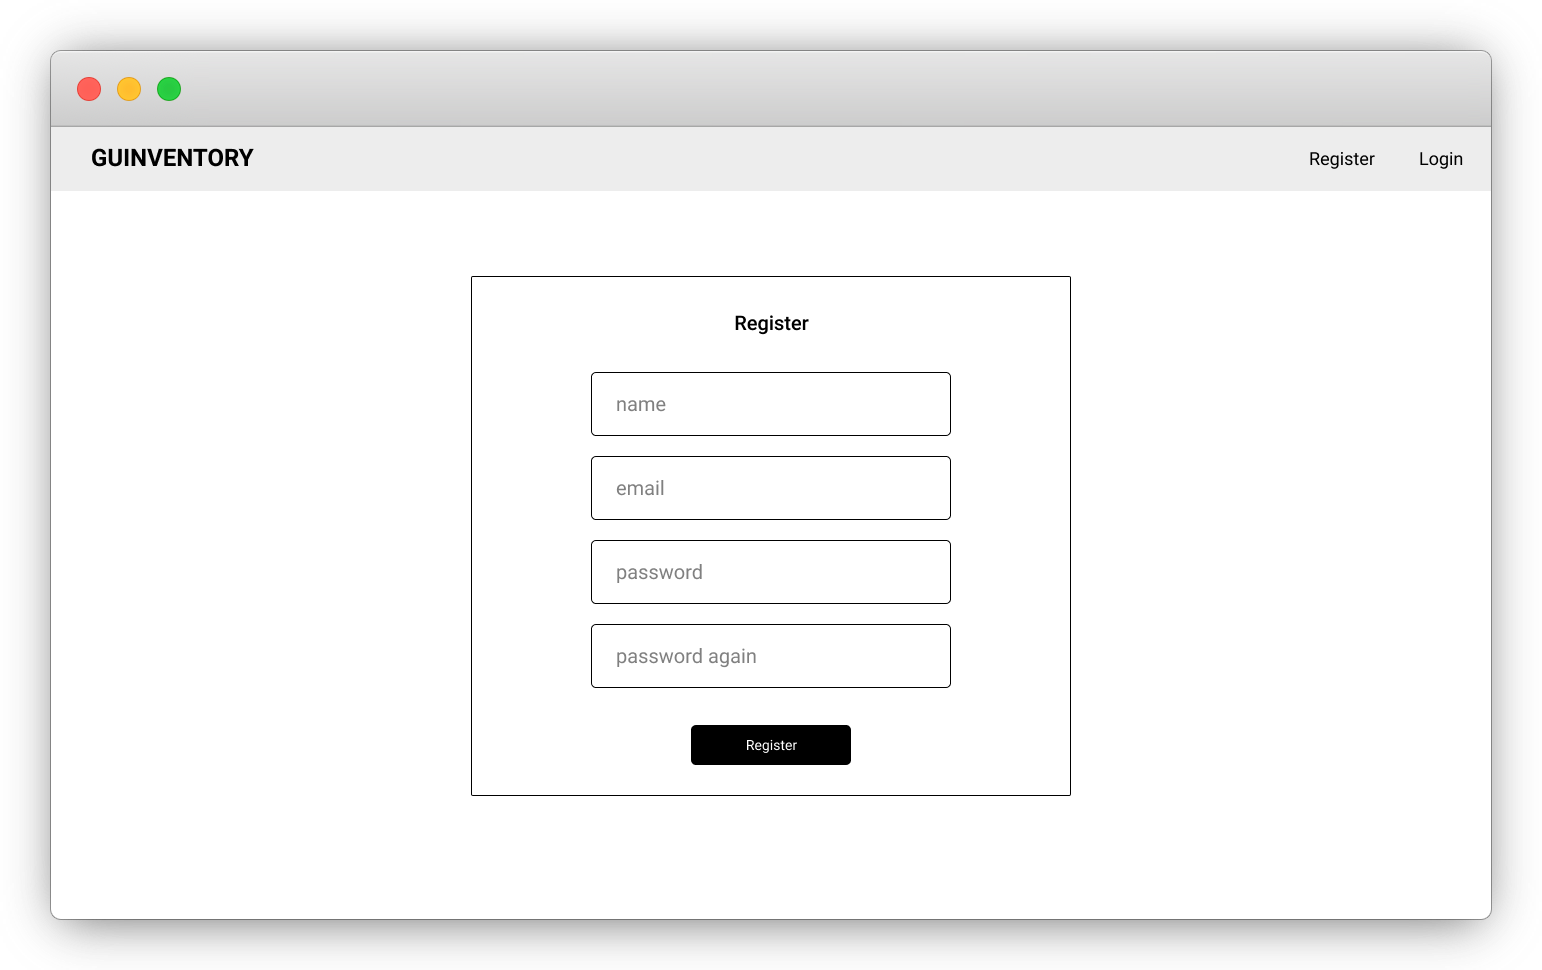
\includegraphics[width=150mm, keepaspectratio]{figures/wireframes/frame_registration.png}
  \caption{Regisztráció wireframe}
  \label{fig:RegistrationWireframe}
\end{figure}


\section{Keresés}
A keresést, annak érdekében, hogy az alkalmazás bármely részéről könnyedén elérhető legyen a felső navigációs sávba helyeztem el.
A wireframe (\refstruc{fig:SearchWireframe}) alapján látszik, hogy kereséskor egy legördülő listában jellennek meg az eredmények, így az aktuális oldal elhagyása nelkél láthatjuk a keresett eszköz helyét.
\begin{figure}[!ht]
  \centering
  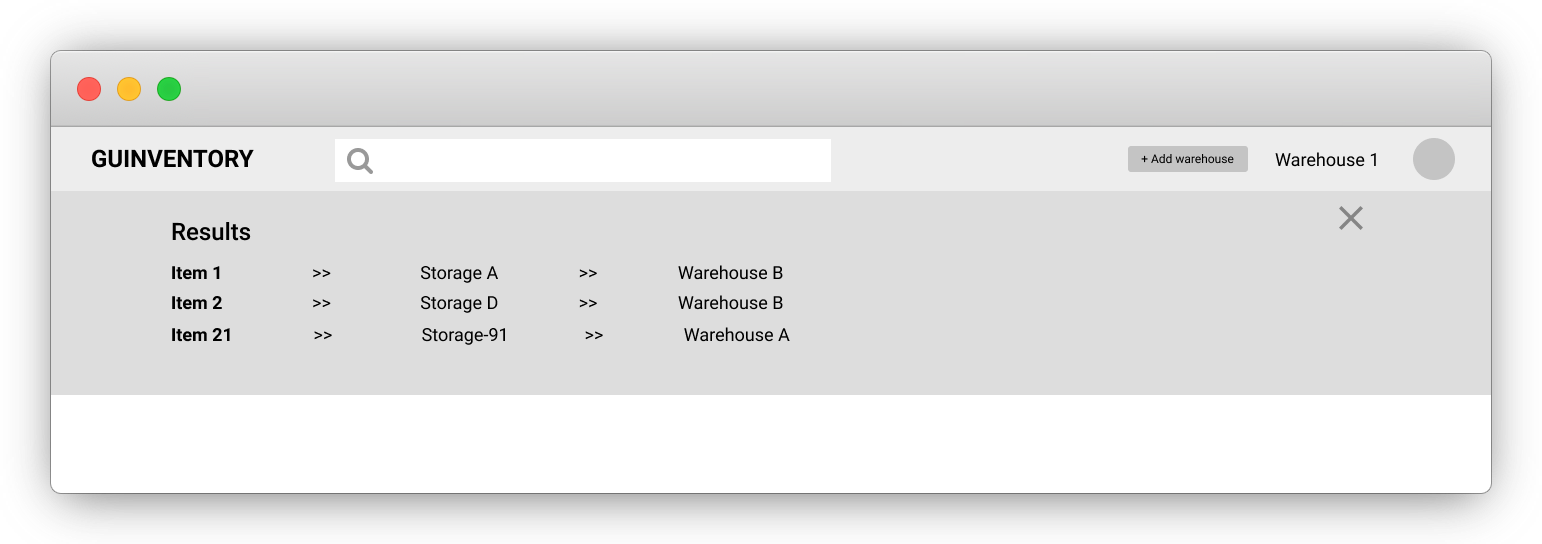
\includegraphics[width=150mm, keepaspectratio]{figures/wireframes/search.png}
  \caption{Keresés wireframe}
  \label{fig:SearchWireframe}
\end{figure}


\section{Raktár nézet}
A raktár oldalán (\refstruc{fig:WarehouseWireframe}) láthatunk egy térképes nézetet és egy listát is a tárololókról. 
A térképes nézeten a kurzort a tároló fülé mozgatva megjelnítjük annak nevét a könnyebb azonosítás érdeképben.

Ezen felül a navigációs bárban láthatjük az éppen kiválasztot raktárat, ahol egy legördülő menü segítségével azonnal választhatunk másik raktárat is, amennyiben több raktárhoz is van hozzáférésünk.
A raktár választó mellett megjelenítünk egy gombot, amellyel új tárolót hozhatunk létre.
\begin{figure}[!ht]
  \centering
  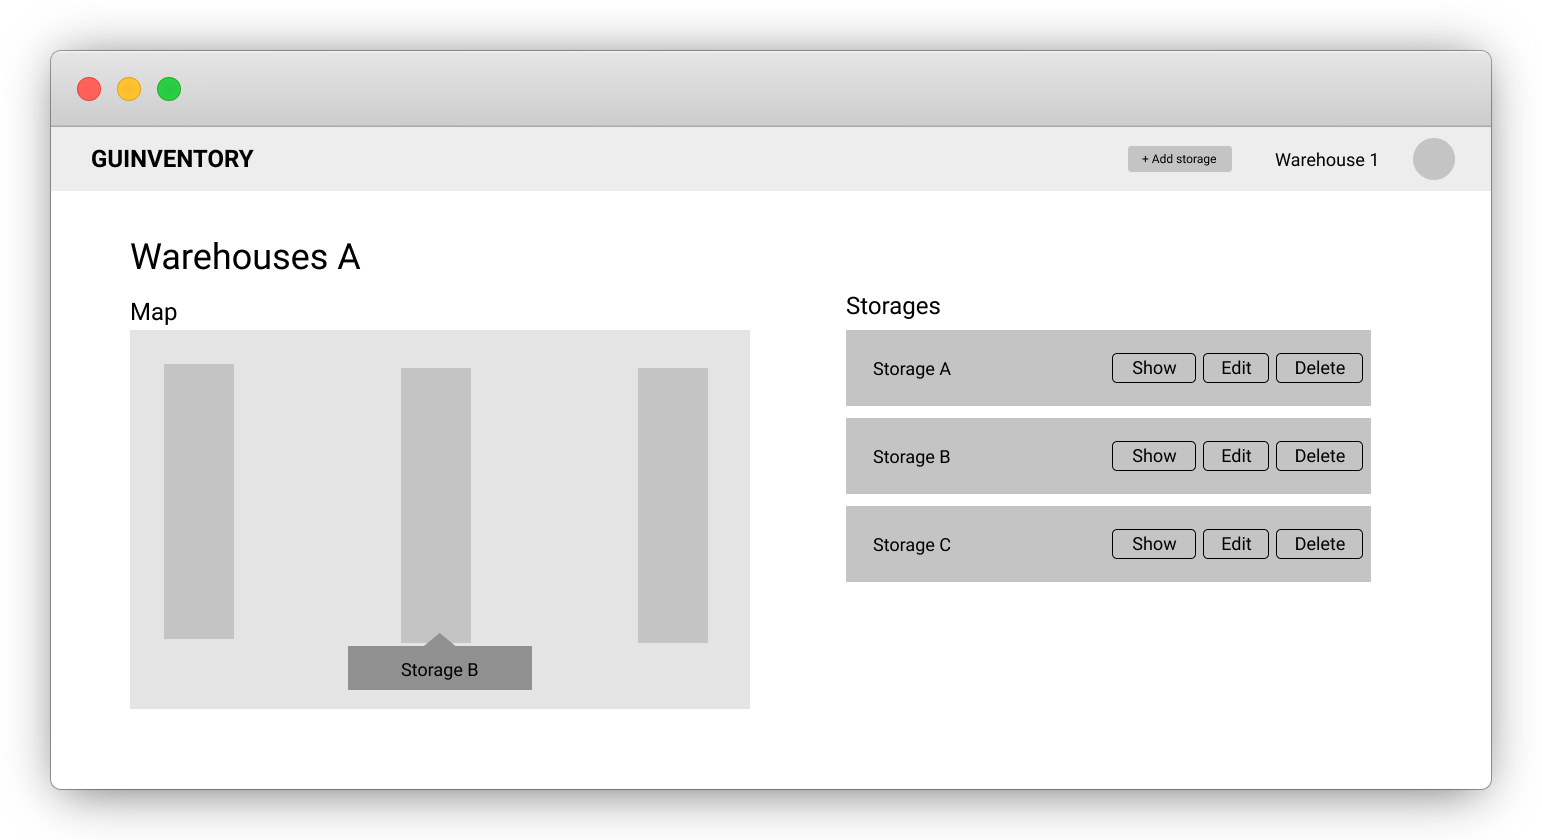
\includegraphics[width=150mm, keepaspectratio]{figures/wireframes/frame_warehouse.png}
  \caption{Raktár wireframe}
  \label{fig:WarehouseWireframe}
\end{figure}

\section{Tároló nézet}
A tároló nézete (\refstruc{fig:StorageWireframe}) nagyban hasonlít a raktáréhoz, azonban itt kiegészítésképt a térkép felett megjelenítünk egy másik tárolót.
Ez a feladatspecifikációban megkövetelt tárolók közötti eszköz mozgatását teszi lehetővé.

A navigációs bárban itt is megjelenítjük a raktár válaztó gombot, azonban a tároló létrehozása helyett, itt az eszköz felvétele gombot találhatjuk.

\begin{figure}[!ht]
  \centering
  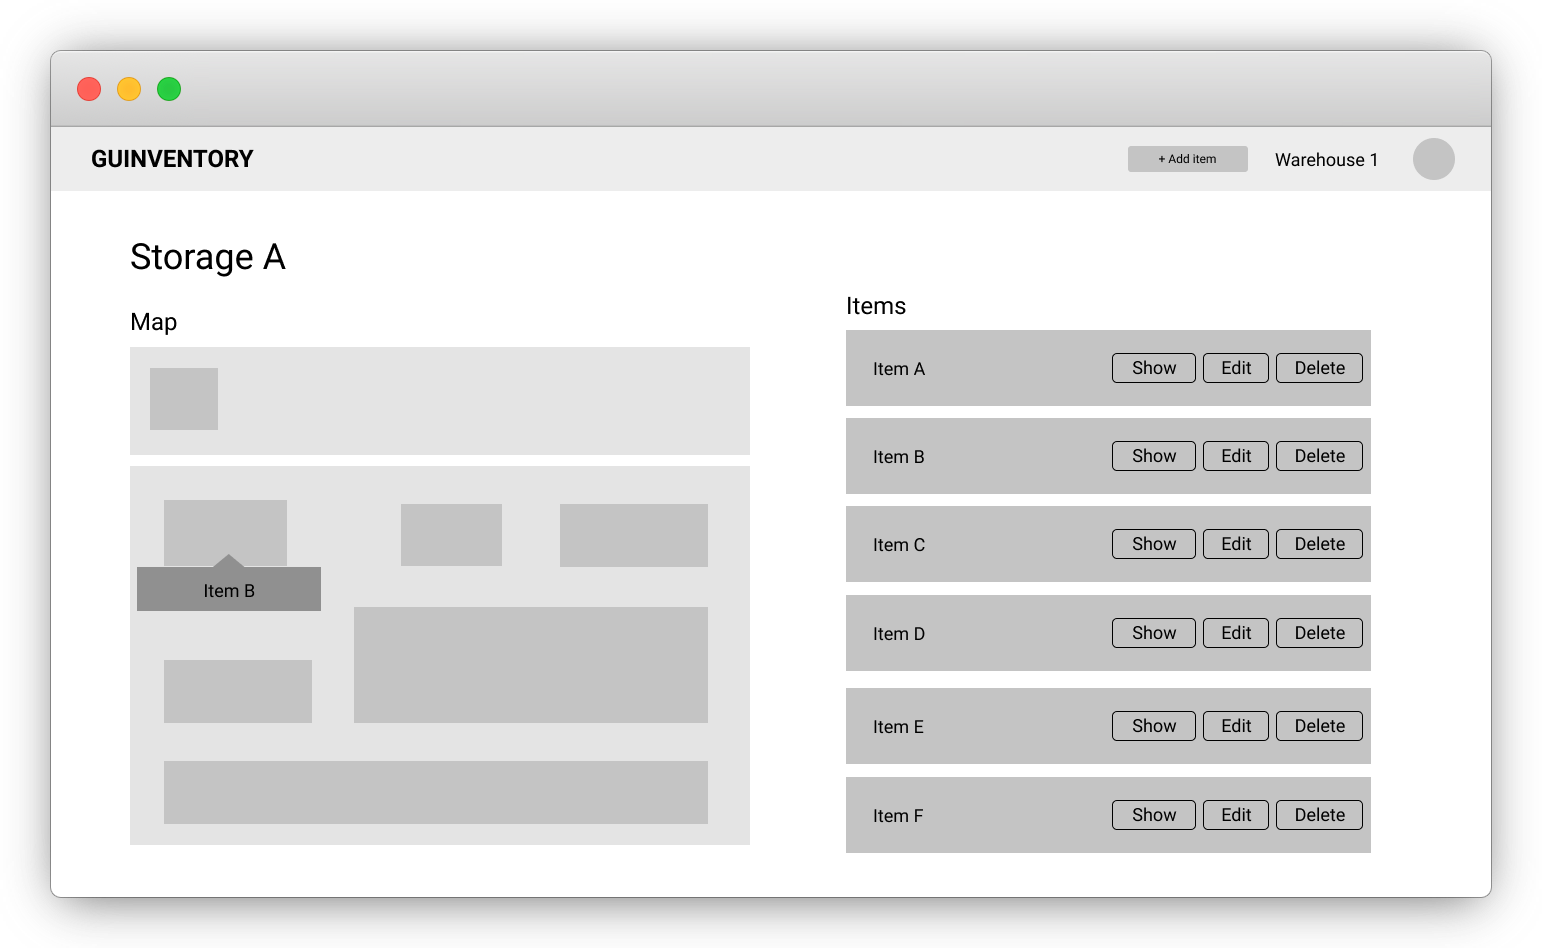
\includegraphics[width=150mm, keepaspectratio]{figures/wireframes/frame_storage.png}
  \caption{Tároló wireframe}
  \label{fig:StorageWireframe}
\end{figure}
  
%----------------------------------------------------------------------------
\chapter{Választott technológiák}
%----------------------------------------------------------------------------

Annek a fejezetnek a keretein belül a felhasznált technológiák kiválasztásának szempontjait szeretném bemutatni. 
Elöszőr a frontend technológiát választottam ki úgyanis az alkalmazásnak ez a része a bonyolultabb a raktár térképek kezelése miatt.
%----------------------------------------------------------------------------

\section{Frontend}

A piacon jelenleg 3 meghatározó keretrendszer/könyvtár érhető el, melyek segítségével webes alkalmazások felhasználói felületét készíthetjük el.

Ezek az Angular, a React és a Vue. 
Bár mind a három keretrendszer célja ugyan az mégis nagy eltéréseket tapasztalhatunk a kódbázisban, felépítésben és a fejlesztúk filozofiájában.
%----------------------------------------------------------------------------

\subsection{Angular}

Az Angular a Google által 2010-ben elinditott és a mai napig általuk karbantartott keretrendszer.
Filozofiája az, hogy egy általános felhasználásra felkészített alapot ad. 
Tartalmazza a formok validációját, az állapot kezelést, a routing-ot és a felhasználói input-ok kezelését és ezen kivül még rengeteg más olyan dolgot is, ami hasznos lehet egy webalkalmazás fejlesztéséhez.
%----------------------------------------------------------------------------

\subsection{React}

Az Angular-hoz hasonlóan a React mögött is egy nagy cég áll.
A Facebook 2013 óta fejleszti és tartja karban a keretrendszert.
Az Angularral szemben a React, filozofiája szerint csak egy könnyű sulyú keretet ad. 
Emiatt talán nem is nevezhetjük keretrendszernek, sokkal inkább csak egy könyvtár. 
Azonban ennek és a fejlesztők által implementált virtuális DOM-nak köszönhetően sokkal jobb sebesség érhető el vele.
Természetesen az, hogy csak egy keretet ad nem okoz semmilyen hátrányt.
Ugyanis rengeteg hivatalos csomag érhető el hozzá, melyek megvalósítják az Angular által is nyujtott megoldásokat.
%----------------------------------------------------------------------------

\subsection{Vue}
A három keretrendszer közül a legújabb és legkevesebb fejlesztői erőforrással rendelkező opció.
A fejlesztését 2014-ben kezdte a Google egyik korábbi mérnöke, aki a mai napig szerves részét képezi a projektnek.
Filozofiáját tekintve a korábban tárgyalt két rendszer között helyezhető el. Többet tartalmaz, mint a React de korán sem annyit, mint az Angular. Itt is találkozhatunk a virtuális DOM-mal melynek köszönhetően nagyon gyors a működése.
Az összehasonlított keretrendszerek közül ezzel a legkönnyeb elkezdeni a fejlesztést, egy egyszerű alkalmazás elkészítése nem igényel sok ismeretet a HTML, CSS és JavaScript-en kívül. Természetesen komplex alkalmazásokat is készíthetünk vele, ipari környezetben is remekül megállja a helyét. 
%----------------------------------------------------------------------------

\subsection{Trendek}
A döntés meghozása elött végeztem egy kisebb kutatást a napjainkban tapasztalható trendekről. Ehhez a Google Trends és az NPM Trends szolgáltatásait vettem igénybe. Előbbi segitségével a Google keresések számát tudjuk összehasonlítani, míg utóbbival az NPM csomagkezelő oldalról történő letöltések számát.

\begin{figure}[!ht]
  \centering
  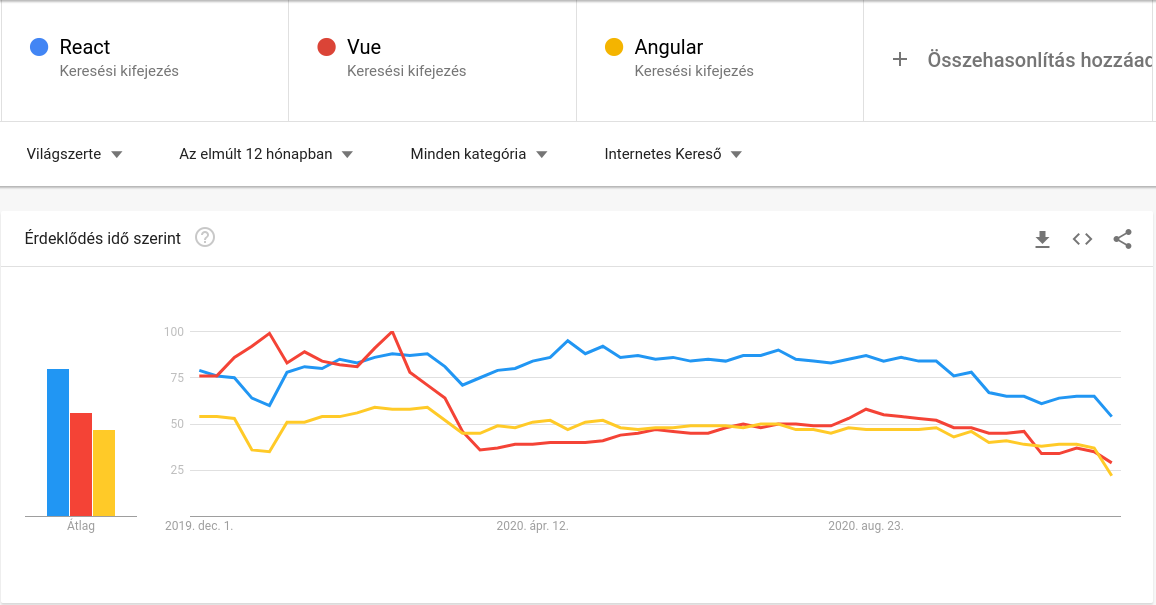
\includegraphics[width=150mm, keepaspectratio]{figures/google_trends.png}
  \caption{Google Trends - keresések összehasonlítása.}
  \label{fig:GoogleTrends}
\end{figure}

A Google keresések alapján a korábbi években az Angular egyértelműen uralta a piacot, azonban a vezető szerepet mára már átvette tőle a React, ahogy az a grafikonon (\refstruc{fig:GoogleTrends}) is látszik.

\begin{figure}[!ht]
  \centering
  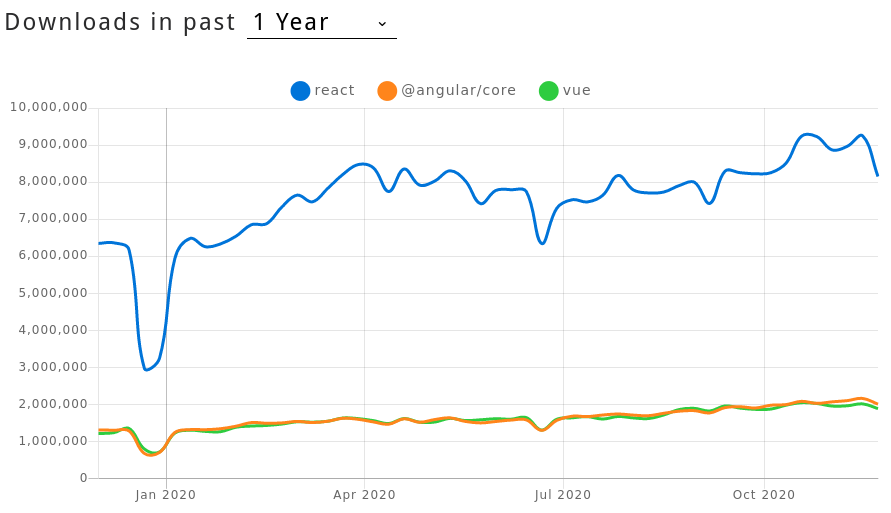
\includegraphics[width=150mm, keepaspectratio]{figures/npm_trends.png}
  \caption{NPM Trends - letöltések összehasonlítása.}
  \label{fig:NPMTrends}
\end{figure}

A Google keresések nem mutattak szignifikáns különbséget, azonban az NPM letöltések számában már jelentős eltéréseket tapasztalhatunk. A grafikonról (\refstruc{fig:NPMTrends}) könnyedén leolvasható, hogy több, mint 4-szer annyi a letöltések száma a React esetén, mint a másik 2 keretrendszernél.
%----------------------------------------------------------------------------

\subsection{Konkluzió}
A fent felsoroltakat alapul véve végül a React-re esett a választásom. A virtuális DOM és az aktív fejlesztői közösség hatalmas elönyt jelent a fejlesztés során. A döntést segítette, hogy ezzel a keretrendszerrel már volt szerencsém dolgozni és pozitív élmény volt.
%----------------------------------------------------------------------------

\section{Backend}

A kliens oldali technológia kiválasztása után a szerver oldali keretrendszer kiválasztására keürlt sor.
Itt sokkal több népszerű és az iparban is használt keretrendszer érhető el. Ilyen például a DotNet, a Spring, a Laravel, a Ruby on Rails, a Django és rengeteg rajtuk kívűl. Ezek összehasonlítása nagyon nehéz, így megpróbáltam egyszerűsíteni a folyamatot. Az elsődleges szempont a kiválasztás során az, hogy a választott frontend technológiával a legegyszerűbben és a legjobban tudjon egyött működni. Természetesen a felsorolt és a nem felsorolt keretrendszerek is működnek React-tel probléma nélkül. Azonban egy kiemelkedik közülük azáltal, hogy a programozási nyelv azonos frontend és backend oldalon is. Ez a NodeJS. Az azonos programozási nyelv felveti a kódmegosztás lehetőségét is a két komponens között. 
%----------------------------------------------------------------------------

\subsection{NodeJS}
A NodeJS története több, mint 11 éve indult Ryan Dahl keze által. A projekt a Google által fejlesztet V8 JavaScript motor segítségével teszi lehetővé JavaScript futtatását web böngészőn kívül, így lehetővé téve a nyelv felhasználását backend oldalon is. A NodeJS gyors ütemben fejlödött, 2011-ben már a Microsoft is kivette a részét a fejlesztésből napjainkra pedig az egyik legnépszerűbb technológia webes környezetben.
%----------------------------------------------------------------------------

\section{Kommunikációs megoldások}

A frontend és a backend technológiák kiválasztása után a következő lépés a köztük történő kommunikáció mikéntjének eldöntése volt.
Itt szerencsémre sokkal kevesebb opció közül kellett választanom. Napjainkban két fő irányvonal figyelhető meg. Ezek a REST API és a GraphQL.
%----------------------------------------------------------------------------

\subsection{REST API}
A REST feloldása REpresentational State Transfer, ami magyarra fordítva Reprezentatív Állapot Átvitel. Ez - ahogy a nevéből is következtetni lehet - probálja kifejező módon átvinni az adatot a kliens és a server alkalmazások között.
Ezt úgy valósítja meg, hogy ajánlást tesz a végpontok nevére és típusára rendeltetésük szerint.

\begin{table}[ht]
	\footnotesize
	\centering
	\begin{tabular}{ l c c l }
		\toprule
		Művelet angolul & Művelet magyarul & HTTP üzenet típusa & Végpont \\
		\midrule
		Create & Létrehozás & POST & /users \\
		Read & Megtekintés & GET & /users/:id \\
		Update & Módosítás  & POST & /users/:id \\
		Delete & Törlés  &  DELETE & /users/:id \\
		List & Listázás  & GET & /users \\
		\bottomrule
	\end{tabular}
	\caption{Példa egy entitáson végezhető müveletekre a REST API elvei szerint}
	\label{tab:RESTTable}
\end{table}
%----------------------------------------------------------------------------

\subsection{GraphQL}

A graphQL egy lekérdező nyelv, amely a jelenleg elterjedt REST API-s megoldásokat próbálja leváltani/kiegészíteni. A megszokott REST API-val ellentétben GraphQL-nél csak egyetlen egy végpont létezik, valamint csak POST típusú HTTP kéréseket használunk. 

Az összes kérést erre a végpontra küldjük a megfelelő tartalommal, melyet a POST kérés törzsében (body) helyezünk el.

A bevett REST API-s megoldással szembeni hatalmas előnye, hogy mindig azt kapjuk amit kérünk. A POST kérés törzsében elhelyezett GraphQL operation pontosan meghatározza, hogy milyen entitások milyen tulajdonságait szeretnénk visszakapni. Ez a GraphQL operation nagyon hasonlít a JSON formátumra, azonban egy-két dologban eltér attól. Lehetőségünk van több entitásból is adatot lekérni egyetlen kéréssel, így csökkentve a HTTP üzenetek számát.

A kéréseket minden esetben egy (vagy több) úgynevezett resolver szolgálja ki nekünk. 
A resolverekből 3 fő típust különböztetünk meg Query, Mutation és Subscription.

\subsubsection{Query}
Adatok lekérésére szolgál
  
\subsubsection{Mutation}
Ahogy a nevéből is következtethetünk rá főként adatok módosítására és létrehozására szolgál
  

\subsubsection{Subscription}
A standard GraphQL implementáció tartalmazza a websocket kommunikációt is. A subscription-ök segítségével lehetősége van a kliensnek feliratkozni bizonyos eseményekre, melyek bekövetkeztéről azonnal értesül socket kapcsolaton keresztül.
%----------------------------------------------------------------------------

\subsection{Konkluzió}
A fent leírt szempontokat figyelembe véve a végső választásomat a GraphQL mellett tettem le.
Tanulmányaim során rengetegszer találkoztam REST API-t használó vagy annak megvalósításák követelő feladattal, így ezen opció választása esetén nem mélyítettem volna el a tudásomat egy kevésbé ismert, azonban mégis remek technológiában.
%----------------------------------------------------------------------------

\section{Adatbázis}
Az alkalmazás nem rendelkezik olyan követelménnyel, amely komoly adatbázis műveletet igényel.
Ezért a választás szempont elsődlegesen az volt, hogy a már kiválasztott technológiákkal egyűtt a lehető legkényelmesebb és legjobb fejlesztési élményt nyújtsa. Ennek követelménye az volt, hogy adatbázisok helyett ORM rendszerek összehasonlítását kezdtem el.
Az ORM egy absztrakciós réteget helyez az adatbázis és az alkalmazás közé, így elfedve a lekérdező nyelvet, ez nagyobb biztonságot és gyorsabb fejlesztést eredményez.

%----------------------------------------------------------------------------
\subsection{TypeORM}

%----------------------------------------------------------------------------

\subsection{Sequelize}
%----------------------------------------------------------------------------

%----------------------------------------------------------------------------
\subsection{Mongoose}
A Mongoose ORM a mongoDB kezeléséhez létrejhozott csomag. A 
%----------------------------------------------------------------------------

\subsection{Prisma}

%----------------------------------------------------------------------------

\subsection{Konkluzió}
Habár a trendek (\refstruc{fig:ORMTrends}) alapján a Prisma jócskán el van maradva népszerűségben az összehasonlításban részt vett többi ORM-től mégis erre esett a választásom.
A korábban felsorolt elönyök és a növekvő népszerűség miatt úgy érzem, hogy a lemaradása egyedül az újdonságának köszönhető.

Tekintve, hogy fejlesztése még mindig egy korai stádiumban van az adatbázis kezelők listája szükös.
A fejlesztés kezdetekor csak PostgreSQL, MySQL és SQLite volt támogatott, utobbi kisebb hiányoságokkal.
A dolgozat írása közben bejelentették a MSSQL támogatást is. 
A választáskor a MySQL és PostgreSQL között kellett döntenem.
Az adatbázisom bonyolultsága nem lesz túl nagy, így személyes preferencia alapján a PostgreSQL mellett döntöttem.
%----------------------------------------------------------------------------

\begin{figure}[!ht]
  \centering
  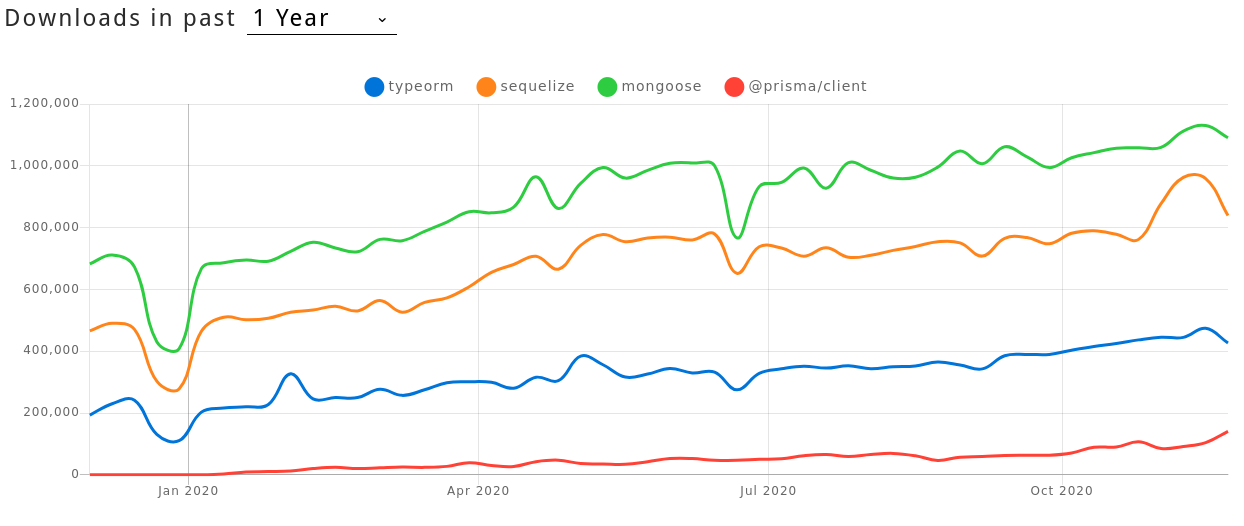
\includegraphics[width=150mm, keepaspectratio]{figures/orm_npm_trends.png}
  \caption{NPM Trends - ORM-ek letöltésének összehasonlítása.}
  \label{fig:ORMTrends}
\end{figure}

%----------------------------------------------------------------------------
\section{Közös technológiák}
%----------------------------------------------------------------------------
Ahogy azt a korábbi fejezetben is említettem a NodeJS-nek hála a backend és a frontend oldali alkalmazás azonos nyelvet használ, a JavaScript-et.
A JavaScript egyik nagy hátránya az, hogy gyengén típusos nyelv (természetesen ezt bizonyos esetekben tekinthetjük elönynek is). Ennek a megoldására JavaScript helyett TypeScript-et használtam az alkalmazás megvalósításához.

%----------------------------------------------------------------------------
\subsection{TypeScript}
%----------------------------------------------------------------------------

A TypeScript egy - a Microsoft által fejlesztett - nyílt forráskódú nyelv, amely JavaScript-et egészíti ki statikus típus definíciókkal. Mondhatjuk, hogy a JavaScript egy superset-je.

A típusok segítségével hamarabb észrevehetjük a hibákat az alkalmazásunkban. Azonban fontos megjegyezni, hogy a típusok definiálása opcionális, ezért TypeScript mellett érdemes valamilyen linter-t használni, amely figyelmezteti a programozót ha elmulasztja a típusdefiníciók használatát. 
Minden érvényes JavaScript kód egy érvényes TypeScript kód is, ez részben az elhagyható típusdefiníciók miatt igaz.

Annak érdekében, hogy probléma nélkül futtathassuk a TypeScript kódunkat a böngészőkben minden kódot JavaScript-re transzformálunk. Erre több megoldás is létezik, ilyen például a Babel vagy a TypeScript complier.

A NodeJS-nek köszönhetően használhatjuk backend oldali nyelvként is, így a frontend és a backend közös nyelvet használhat, amely akár a kódmegosztás lehetőségét is felveti.

%----------------------------------------------------------------------------
\chapter{Architektúra}
%----------------------------------------------------------------------------
Az alkalmazás 3 fő részre bontható frontend, backend valamint adatbázis.
E három réteg együttesen felel azért, hogy a felhasználó böngészőn keresztül érkező interrakcióit kezelje és az állapotot tárolja.
%----------------------------------------------------------------------------

\section{Adatbázis séma}
Az adatbázis migrációját nem kellett manuálisan végrehajtanom hála a Prisma-nak. 
A Prisma - amellett, hogy kezeli a migrációkat - egy absztrakciós réteget ad az adatbázisunk és az alkalmazásunk közé olyan szinten, hogy teljesen elfedi az adatbázist a fejlesztő elöl.

Ennek ellenére mégis relációs adatbázist terveztem, majd ezt ültettem át a Prisma által kíván sémába.
Tanulmányaim során ezzel a tervezési metodikával találkoztam és olyannyira rögzült, hogy elöszőr nehéz volt kicsit más szemszögből vizsgálni a problémát.

\begin{figure}[!ht]
  \centering
  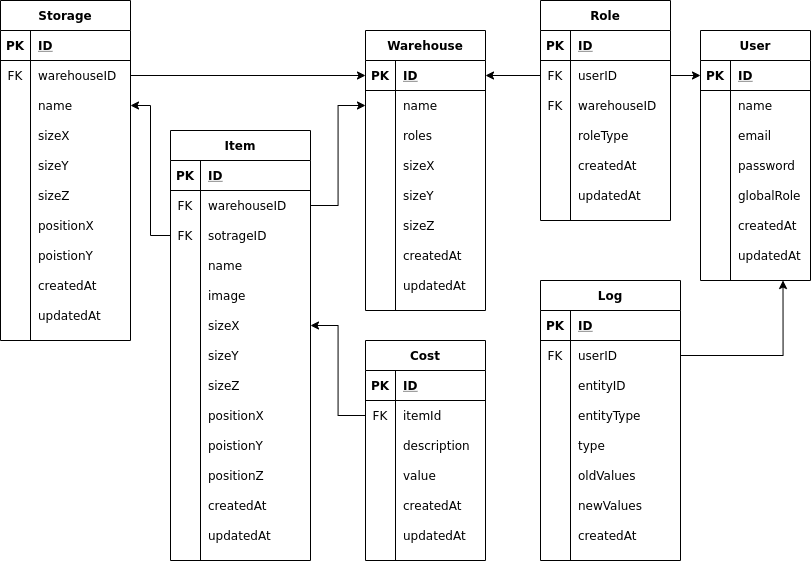
\includegraphics[width=150mm, keepaspectratio]{figures/db.png}
  \caption{Adatbázis séma}
  \label{fig:backend}
\end{figure}

%----------------------------------------------------------------------------

\section{Backend felépítése}
Az alkalmazás üzleti logikáját megvalósító rész egy NodeJS-re épülő rendszer.
Az alkalmazás egyetlen egy végpontot ajánl a kliensek számára.
A kéréseket egy express server fogadja, a feldolgozásának mikéntjéről pedig egy Apollo server gondoskodik, itt történik meg a GraphQL elemzése és ez alapján a megfelelő kódrészlet futtatása.
Az Apollo server lehetőséget nyújt middelware-ek definiálsára, melyek minden kérés kiszolgálása elött lefutnak.
Erre a lehetőségre épít a GraphQL Shield nevű könyvtár, aminek segítségével minden egyes GraphQL műveletre megadhatünk ahhoz szükséges előfeltételeket egyszerű szabályok segítségével.
Ilyen szabályokkal valósítottam meg a teljes authorizációt és az authentikáció ellenörzését is.

\begin{figure}[!ht]
  \centering
  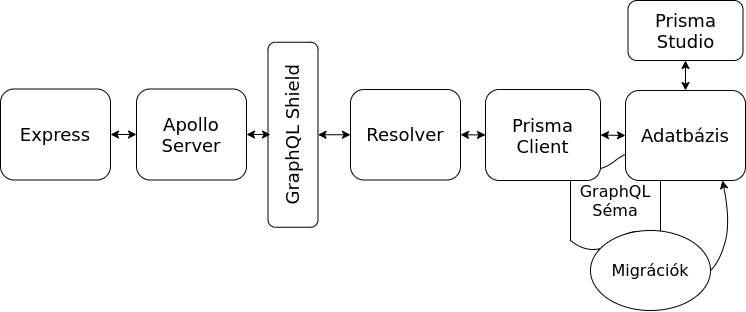
\includegraphics[width=150mm, keepaspectratio]{figures/backend.png}
  \caption{Backend felépítése}
  \label{fig:backend}
\end{figure}

A megfelelő kódrészlet és a middelware-ek futtatása után, a Prismán keresztül az adatbázishoz fordulunk adat lekérés vagy modósítás miatt.

Az ábrán (\refstruc{fig:backend}) világosan látszik, hogy a Prisma által nyújtott studio az adatbázishoz csatlakozik, így az általunk írt üzleti logika nem fog érvenyesülni.
Fontos, hogy az itt végrehajtott modósítások nem várt működéshez is vezethetnek.

%----------------------------------------------------------------------------

\section{Frontend felépítése}

\begin{figure}[!ht]
  \centering
  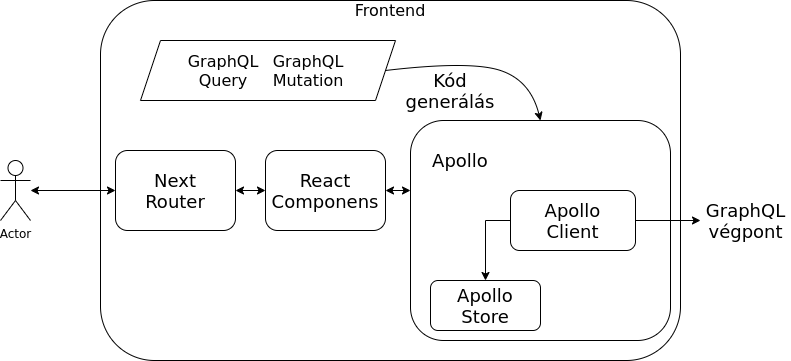
\includegraphics[width=150mm, keepaspectratio]{figures/frontend.png}
  \caption{Frontend felépítése}
  \label{fig:frontend}
\end{figure}

Ahogy azt a korábbi fejezetekben taglaltam a kliens alkalmazás megvalósításához React-et azon belül pedig NextJS-t használtam.
A backendhez csatlakozást az Apollo Client könyvtárral oldottam meg. 
Az Apollo Client és az Apollo Server együtt egy nagyon jól és könnyen használható rendszert alkotnak.
A Client megkapja a Server-től a GraphQL sémát, így fejlesztés közben kódkiegészítéssel és tipus ellenörzéssel írhatjuk a lekérdezéseinket.
Ezen felül lehetőségünk nyílik kódgenerálásra is.
A megírt GraphQL Query és GraphQL Mutation kódokból React hook-okat kapunk, melyekben az állapot- és a típusokkezelés is megvalósított

%----------------------------------------------------------------------------

\section{Architektúra összefoglalása}
Tehát a három fő komponense az alkalmazásnak a frontend, a backend és az adatbázis.
A frontend és a backend közötti kommunikáció GraphQL segítségével történik az Apollo Cliens és az Apollo Server között.
A backend és az adatbázis kommunikációja pedig SQL segítségével történik, azonban ezt a Prisma teljesen elfedi.

\begin{figure}[!ht]
  \centering
  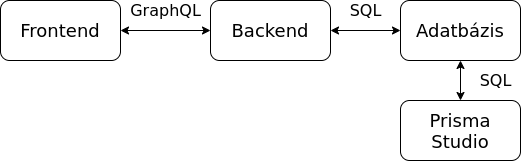
\includegraphics[width=150mm, keepaspectratio]{figures/architecture.png}
  \caption{Teljes alkalmazás felépítése}
  \label{fig:architecture}
\end{figure}
% !TeX spellcheck = hu_HU
%----------------------------------------------------------------------------
\chapter{Fejlesztést segítő eszközök}
%----------------------------------------------------------------------------
A fejlesztés során igyekeztem minél több olyan eszközt használni, ami elősegíti a munkát és javítja a kódminőséget és biztonságot.
%----------------------------------------------------------------------------

\section{Continuous Integration}
A Continuous Integration (rövidítve CI) napjainkban már elengedhetetlen része a fejlesztési folyamatoknak.
Rengetek megoldás létezik, azonban én a GitHub Action mellett tettem le a voksomat.
Ennek oka, hogy a GitHub-ot használtam a verziókezelt kódom tárolására, így kézen fekvő volt ennek a megoldásnak az alkalmazása.

Az alkalmazást 2 külön repository-ban kezeltem, hogy jobban elkülönüljön a frontend és a backend kódja.
Ennek a hátránya az volt, hogy bár ugyan azon nyelvet használja a két repository mégis kétszer kellett implementálnom a GitHub Action-öket.

Az action-ök létrehozását egyszerű szöveges formában tehetjük meg. 
A \lstinline|.github/workflows| mappába létrehozott github \lstinline|.yml| és \lstinline|.yaml| kiterjesztésű fájlok automatikusan kiértékelődnek a GitHub Action által.

\begin{figure}[!ht]
  \centering
  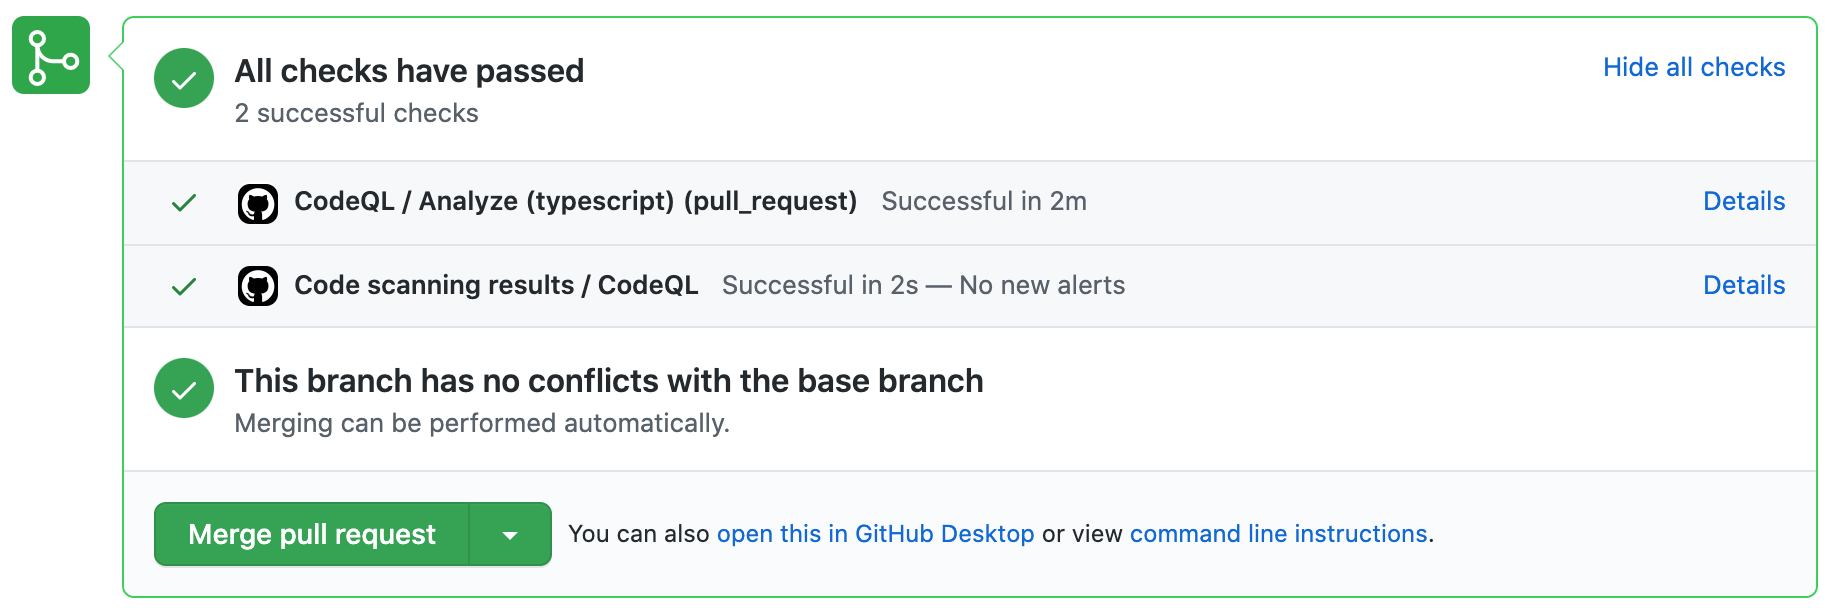
\includegraphics[width=150mm, keepaspectratio]{figures/ci.png}
  \caption{GitHub Action működés közben}
  \label{fig:GitHubAction}
\end{figure}
%----------------------------------------------------------------------------

\subsection{Linter}
A linter egy viszonylag gyors lefutású és kevés erőforrást igénylő action, ezért beállítása szerint bármilyen commit kerül a GitHub repository-ba azonnal elindul.


%----------------------------------------------------------------------------
\subsection{Statikus kódellenörzés}
A statikus kódellenőrzést egy a GitHub által ajánlott megoldással valósítottam meg a CodeQL-lel.
Mivel ez egy több erőforrást igénylő folyamat ezért a futtatása nem történik meg minden commitnál.
Csak ha a főágba történik a commit vagy ha Pull Request-et kezdeményezek, melynek a cél ága a főág.

A képen (\refstruc{fig:securityCheck}) egy a GitHub által észlelt lehetséges sebezhetőség detektálása látható.
A kód analízis során a rendszer észlelte, hogy shell command futtatása történik úgy, hogy annak tartalma környezeti változóból származik.
A figyelmeztetés jelen esetben egy fals riasztás volt, mert a sérülékeny kódrészlet az alkalmazása futása közben nem érhető el, ugyanis a teszt környezet kialakítására szolgál.

\begin{figure}[!ht]
  \centering
  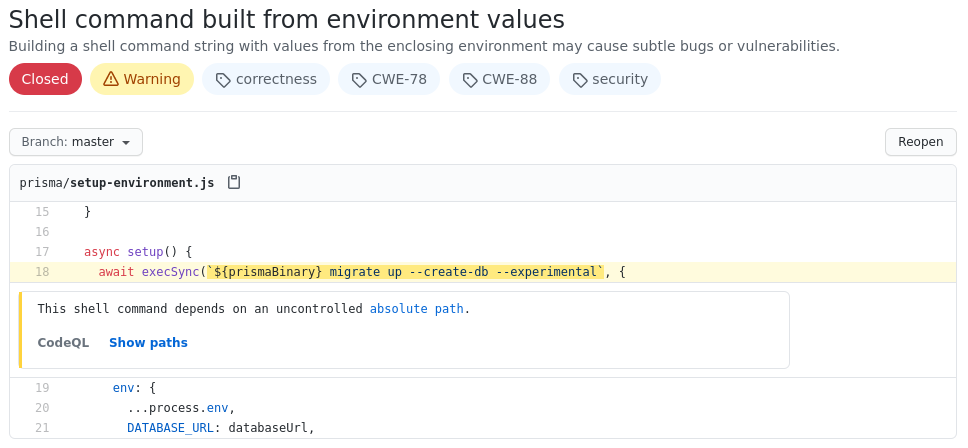
\includegraphics[width=150mm, keepaspectratio]{figures/security.png}
  \caption{Code scanning figyelmeztetés}
  \label{fig:securityCheck}
\end{figure}
%----------------------------------------------------------------------------

\section{Git hook}
Git használata esetén rengeteg eseményhez definiálhatunk úgynevezett hook-okat.
Ezek segítségével bizonyos események után, előtt vagy közben futtathatunk tetszőleges kódot.
Az alkalmazásomban egy linter-t állítottam be a pre-commit hookra, az-az a commit elkészítése előtt minden alkalommal lefut a linter így biztosítva a kódminőségét.

\begin{lstlisting}[style=ES6, caption=Pre-commit hook beállításai]    
"husky": {
  "hooks": {
    "pre-commit": "lint-staged"
  }
},
"lint-staged": {
  "*.ts": [
    "eslint --fix"
  ]
}
\end{lstlisting}
  
%----------------------------------------------------------------------------

\section{Continuous Deployment}
A Continuous Integration melett elengedhetetlen része a fejlesztésnek a Continuous Deployment (röviden CD).
A CD az alkalmazás folyamatos kitelepítését jelenti, hogy a kód felöltése után szinte azonnal elérhető legyen az alkalmazás legfrissebb változata.

%----------------------------------------------------------------------------

\subsection{Heroku}
A backend alkalmazás üzemeltetésére a Heroku szolgáltatásai vettem igénybe.
Webes felületének és GitHub integrációjának köszönhetően nem igényel komoly szakértelmet az alkalmazás elindítása.
Ingyenes keretek között csak egy ág automatikus kitelepítésére van lehetőség, azonban beállítható az is, hogy megvárja a CI kimenetelét és csak sikeres futás után kezdje el a telepítést.
Így elkerülhetjük hibás- vagy biztonsági réseket tartalmazó kódok éles környezetbe jutását.

%----------------------------------------------------------------------------

\subsection{Vercel}
A frontend üzemeltetéséhez a Vercel-t használtam. 
A Herokuhoz hasonlóan remek GitHub integrációval és webes felülettel rendelkezik. 
Lehetőségünk nyílik a Pull Request-ekhez egy előnézeti alkalmazás kitelepítésére is, ezzel elősegítve a csapatmunkában egymás munkájának ellenőrzését.
Ilyenkor a Vercel automatikusan hozzáad egy megjegyzést (\refstruc{fig:vercel}) a Pull Requesthez az előnézeti alkalmazás linkjével.

\begin{figure}[!ht]
  \centering
  
\includegraphics[width=150mm, keepaspectratio]{figures/vercel.png}
  \caption{Vercel megjegyzése Pull Reques-nél}
  \label{fig:vercel}
\end{figure}

%----------------------------------------------------------------------------


% !TeX spellcheck = hu_HU
%----------------------------------------------------------------------------
\chapter{Alkalmazás fejlesztése és működése}
%----------------------------------------------------------------------------

\section{Backend}
A backend architekturális felépítését a korábbi fejezetben már részletesen taglaltam.  
Ebben a fejezetben az egyes rétegek és egyes funkciók megvalósításának bemutatására fektettem a hangsúlyt.
%----------------------------------------------------------------------------

\subsection{GraphQL Playground}
A legtöbb GraphQL server-hez lehetőségünk nyílik valamilyen interaktív GraphQL szerkesztő felület kiszolgálásra is.
Az alkalmazásban én a GraphQL Playground-ot használtam. Ennek a konfigurációt úgy valósítottam meg, hogy éles környezetbe ne szolgálja ki a felületet, csak fejlesztői környezet estén.
Ezt környezeti változók segítségével oldattam meg.

Azon felül, hogy interaktívan, kódkiegészítéssel szerkeszthetjük a GraphQL kódunkat kapunk egy dokumentációt is, amely tartalmazza az elérhető Query-k és Mutation-ök listáját a lehetséges paraméterekkel és a válaszok típusával együtt.
Így a használatával még kényelmesebben készíthetjük el a lekérdezéseinket, melyeknek futtatására is lehetőségünk van.

\begin{figure}[!ht]
  \centering
  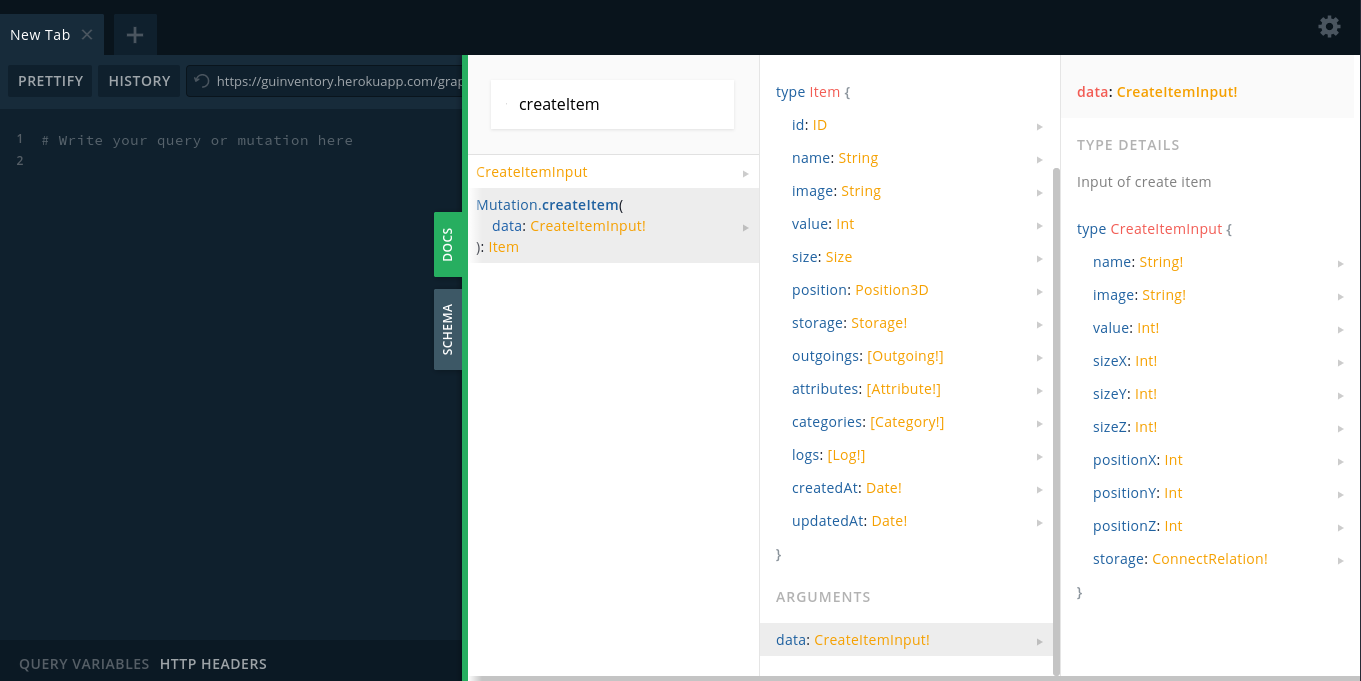
\includegraphics[width=150mm, keepaspectratio]{figures/playground_docs.png}
  \caption{GraphQL Playground Docs}
  \label{fig:playgroundDocs}
\end{figure}
%----------------------------------------------------------------------------

\subsection{Modellek és kapcsolatok}
A modell definiálásakor megadhatunk bármelyiket a sémában szereplő attribútumok közül, azonban fontos figyelni arra, hogy a típusok megegyezzenek a sémában és a modellben.
A kapcsolatokat is egyszerű mezőként kezelhetjük, beállítható továbbá az is, hogy a kapcsolat opcionális vagy kötelező illetve, hogy egy vagy több entitást tartalmazhat.
Lehetőségünk van egyedi attribútumok létrehozására is, amely az adott modell bármely attribútumából származtatható, de tetszőleges kód futtatása is megengedett, így bármilyen származtatott értéket képesek vagyunk felvenni a modelljeinkhez.

Az egyszerűség és teljesség kedvéért a példában a \lstinline|MyModel| felépítésén mutatom be egy modell definiálását.
Az \lstinline|id| és a \lstinline|name| egyszerű, az adatbázisból származó attributumok. A \lstinline|user| egy kapcsolatot reprezentál, pontosan egy darab \lstinline|User|-t tartalmaz. 
A \lstinline|custom| mező egy egyedi attributum, ami az \lstinline|id| elejére egy kettős-keresztet fűz és úgy adja vissza azt.
\begin{lstlisting}[style=ES6, caption={Példa model}]
import { objectType } from '@nexus/schema'

export const MyModel = objectType({
  name: 'MyModel',
  definition(t) {
    t.id('id')
    t.string('name')
    t.field('user', {
      type: 'User',
      nullable: false,
    }),
    t.field('custom', {
      type: 'User',
      nullable: false,
      resolve: ({id}) => `#${id}`
    })
  },
})
\end{lstlisting}
%----------------------------------------------------------------------------

\subsection{Resolver felépítése}
A Mutation-ökhöz és Query-khez tartozó resolverek minden esetben tartalmaznak egy függvényt, amely eldönti, hogy meghívásukkor milyen kódrészlet fusson le.
Ezen felül a használatukhoz szükségünk van metainformációkra is, ezért tartalmaz egy visszatérési típust, hogy pontosan tudjuk milyen típussal térhet vissza, valamint opcionálisan tartalmaz egy argumentum listát, ami meghatározza, hogy milyen paraméterek szükségesek és milyen paraméterek opcionálisak a meghívásához.
A paraméter lista meghatározza a paraméterek típusát is.

Az alábbi példában egy egyszerű létrehozásra láthatunk egy lehetséges implementációt.
A kódrészletben látható, hogy az argumentum lista helyett használhatunk külön definiált bemenetet is, így növelve a kód olvashatóságát.
A resolve függvényben elvégezhetjük a szükséges adatbázis műveletet és meghívhatunk külső függvényeket is.
A csatolt kódban az eszköz létrehozáson felül meghívjunk egy függvényt, amely elkészíti az eseményhez tartozó napló bejegyzést, valamint küldünk egy jelzést az elem létrehozásához.
Ezekre a jelzésekre a GraphQL Playground vagy bármilyen kliens segítségével feliratkozhatunk egy egyszerű websocket kapcsolattal.

\begin{lstlisting}[style=ES6, caption={Eszköz létrehozás resolver}]
t.field('createItem', {
  type: 'Item',
  args: { data: CreateItemInput.asArg({ required: true }) },
  resolve: async (_, { data: { storage, ...rest } }, context: Context) => {
    const item = await context.prisma.item.create({
      data: {
        storage: { connect: storage },
        ...rest,
      },
    })
    await log({
      type: 'CREATE',
      entityId: item.id,
      entityName: 'Item',
      newValues: { storage, ...rest },
      context,
    })
    await publishItemEvent('itemCreated', item, context)
    return item
  },
})
\end{lstlisting}
%----------------------------------------------------------------------------

\subsection{Autentikáció és autorizáció}
Az autentikáció és autorizáció ellenőrzésére a GraphQL Shield-et használtam. 
Ennek segítségével egy egyszerű JavaScript object-tel megadható, hogy egyes Query-k és Mutation-ök esetén, milyen validáció fusson le.
Lehetőséget biztosít egy úgynevezett fallback rule beállítására is, amely minden külön nem specifikált kérésnél fut le.
Ezzel valósítottam meg a bejelentkezett felhasználó validálását.

\begin{lstlisting}[style=ES6, caption={GraphQL Shield}]
export const shield = GQLShield(
   {
     Query: {
       warehouses: isGlobalAdmin,
       logs: isGlobalAdmin,
     },
     Mutation: {
       login: allow,
       register: allow,
     },
   },
   {
     allowExternalErrors: true,
     fallbackRule: fallbackRule,
   },
)
\end{lstlisting}

Az authentikációt JSON Web Token segítségével végzem. 
Sikeres bejelentkezés esetén a backend egy tokent küld a frontend részére, melyet a böngészőbe elmentve a későbbiekben minden kéréshez csatolni tudunk.

\begin{figure}[!ht]
  \centering
  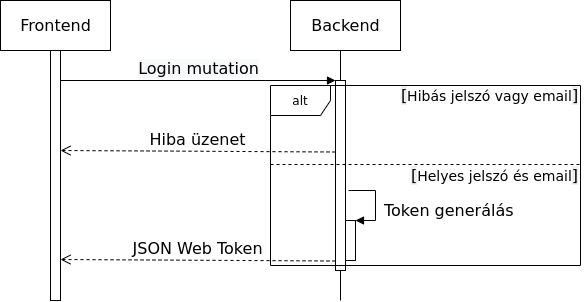
\includegraphics[width=150mm, keepaspectratio]{figures/login.png}
  \caption{JWT Bejelentkezés}
  \label{fig:JWT}
\end{figure}
%----------------------------------------------------------------------------

\subsection{Képek kezelése}
Az alkalmazáson belül lehetőségünk van kép feltöltésre a raktárba vett eszközökről.
A képek tárolására a Google Cloud Storage szolgáltatását használtam. 
A képeket feltöltés előtt base64-es formátumra kódolom át és elküldöm a backend részére.
A backend végzi a kép feltöltését a Google Cloud Storage rendszerébe és eltárolja a kép URL címét az adatbázisba a megfelelő eszköz attribútumai között.
%----------------------------------------------------------------------------

\section{Frontend}

%----------------------------------------------------------------------------

\subsection{Kódgenerálás}
%----------------------------------------------------------------------------

Ahogy az korábban már többször is szóba került az Apollo-nak hála remek kódgenerálási lehetőségeink vannak.
Alább egy példa keretein belül szeretném bemutatni ennek használatát

A GraphQL Mutation-t paraméterekkel ellátva szükséges megírnunk, hogy a kód generátor tudja lehetséges paramétereket. 
\begin{lstlisting}[style=ES6, caption={GraphQL Shield}]
mutation Login($email: String!, $password: String!) {
  login(data: { email: $email, password: $password }) {
    token
  }
}
\end{lstlisting}

A generálást futtatva azonnal használhatjuk az elkészült hook-okat (jelen esetben a useLoginMutation hook-ot).

A hálózati kapcsolat kezelésén felül megkapjuk annak az állapotát is, így tudjuk a felhasználói felület kinézetét a kérés állapotához kötni.
Például töltés esetén egy töltő képernyőt megjeleníteni, vagy a hibákat kezelni.

\begin{lstlisting}[style=ES6, caption={Bejelentkezés kódrészlet}]
const { register, handleSubmit, errors } = useForm<Inputs>()
const [login, { loading }] = useLoginMutation()
const toast = useToast()
const { setAuthToken } = useAuthToken()

const onSubmit = async (inputData) => {
  try {
    const {
      data: {
        login: { token },
      },
    } = await login({
      variables: inputData,
    })
    setAuthToken(token)
    window.location.href = '/'
  } catch (error) {
    toast({
      title: error.message,
      status: 'error',
      duration: 3000,
      isClosable: true,
    })
  }
}
\end{lstlisting}
%----------------------------------------------------------------------------

\subsection{Útvonalválasztás}
NextJS használatával alapértelmezetten fájl alapú útvonalválasztást használhatunk.
Ez azt jelenti, hogy az oldal URL-jét a fájl neve és a szülő mappák nevei határozzák meg.
Lehetőségünk van paraméterek használatára is, ezt szögletes zárójelek közé írt névvel jelezhetjük.
A paramétert ezzel a névvel fogjuk elérni a kódbázison belül is.
Ilyen paraméterrel jelzett adhatunk bármelyik szinten lévő fájlnak, de akár mappának is.

\begin{figure}
	\dirtree{%
      .1 /pages.
      .2 auth.
      .3 login.tsx.
      .3 register.tsx.
      .2 index.tsx.
      .2 warehouse.
      .3 [warehouse\_id].
      .4 edit.tsx.
      .4 editroles.tsx.
      .4 index.tsx.
      .4 storage.
      .5 [storage\_id].
      .6 edit.tsx.
      .6 index.tsx.
      .6 item.
      .7 [item\_id].
      .8 cost.
      .9 [cost\_id].
      .10 edit.tsx.
      .8 edit.tsx.
      .8 index.tsx.
      .7 index.tsx.
      .5 new.tsx.
      .3 new.tsx.
    }
  \caption{Next mappa szerkezet}
  \label{fig:next}
\end{figure}
%----------------------------------------------------------------------------

\subsection{Validáció}
A felhasználótól érkező adatok minden esetben validálva vannak, ehhez a yup csomagot használtam.
A yup segítségével definiálhatunk egy sémát, amelyre a bemenetnek illeszkedni kell. 
Hiba esetén egy hibaüzenetet is generál az egyes mezőkhöz, így visszacsatolást adhatunk a felhasználónak, hogy melyik adat hibás és miért.
Amennyiben szeretnék eltérni az alapértelmezett beállításoktól, a hibaüzeneteket szövegezését a séma definiálással együtt adhatjuk meg.

\begin{lstlisting}[style=ES6, caption={Esköz validációs séma}]
import * as yup from 'yup'

export const itemSchema = yup.object().shape({
  name: yup.string().required(),
  image: yup.string().required(),
  value: yup.number().required().typeError('Must be a number'),
  positionX: yup.number().required().typeError('Must be a number'),
  positionY: yup.number().required().typeError('Must be a number'),
  positionZ: yup.number().required().typeError('Must be a number'),
  sizeX: yup.number().required().typeError('Must be a number'),
  sizeY: yup.number().required().typeError('Must be a number'),
  sizeZ: yup.number().required().typeError('Must be a number'),
})
\end{lstlisting}

A formok elküldését egy React hook-kal valósítottam meg.
A hook visszaadja a hibákat és lehetőséget biztosít a form újra-beállítására is.
Minden beviteli mezőt regisztrálni kell a form hook-ba, így biztosítva azok elérését.

\begin{lstlisting}[style=ES6, caption={Regisztrációnál használt form hook}]
const { register, handleSubmit, reset, errors } = useForm<Inputs>({
  resolver: yupResolver(itemSchema),
})
\end{lstlisting}

A hibákat egy JavaScript objektumban kapjuk meg, melynek a kulcsa minden esetben az adott beviteli mező neve.

\begin{lstlisting}[style=ES6, caption={Form}]
<form onSubmit={handleSubmit(onSubmit)}>
  <FormControl mb={4} isInvalid={!!errors.name}>
    <FormLabel htmlFor="name">Name</FormLabel>
    <Input name="name" type="text" ref={register} />
    <FormErrorMessage>{errors.name?.message}</FormErrorMessage>
  </FormControl>
  ...
</form>
\end{lstlisting}

%----------------------------------------------------------------------------

\subsection{Felhasználói felület}
A felhasználói felületet a ChakraUI könyvtár segítségével készítettem el.
A Chakra hála az összes általános komponens egy szép és minden lehetséges állapotra felkészített változatban rendelkezésemre állt.

\begin{figure}[!ht]
  \centering
  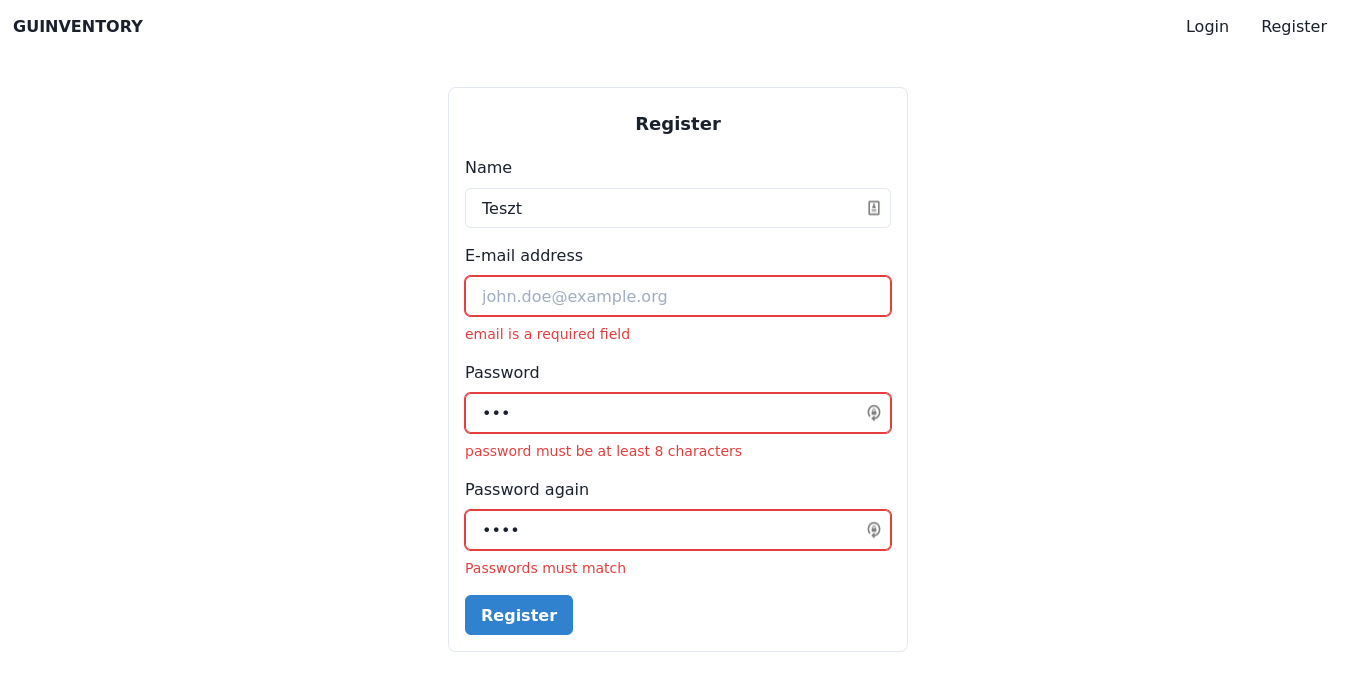
\includegraphics[width=150mm, keepaspectratio]{figures/reg.png}
  \caption{Regisztrációs oldal}
  \label{fig:reg}
\end{figure}

A regisztrációs oldalon (\refstruc{fig:reg}) láthatjuk a beviteli mezőket különböző állapotban.
Hibásan kitöltött mező esetén felhasználó azonnali visszajelzést kap a hibás adatról.
Javítás után a hibaüzenet automatikusan eltűnik, amint megfelelő formátumú adatot gépelt be a felhasználó.

\begin{figure}[!ht]
  \centering
  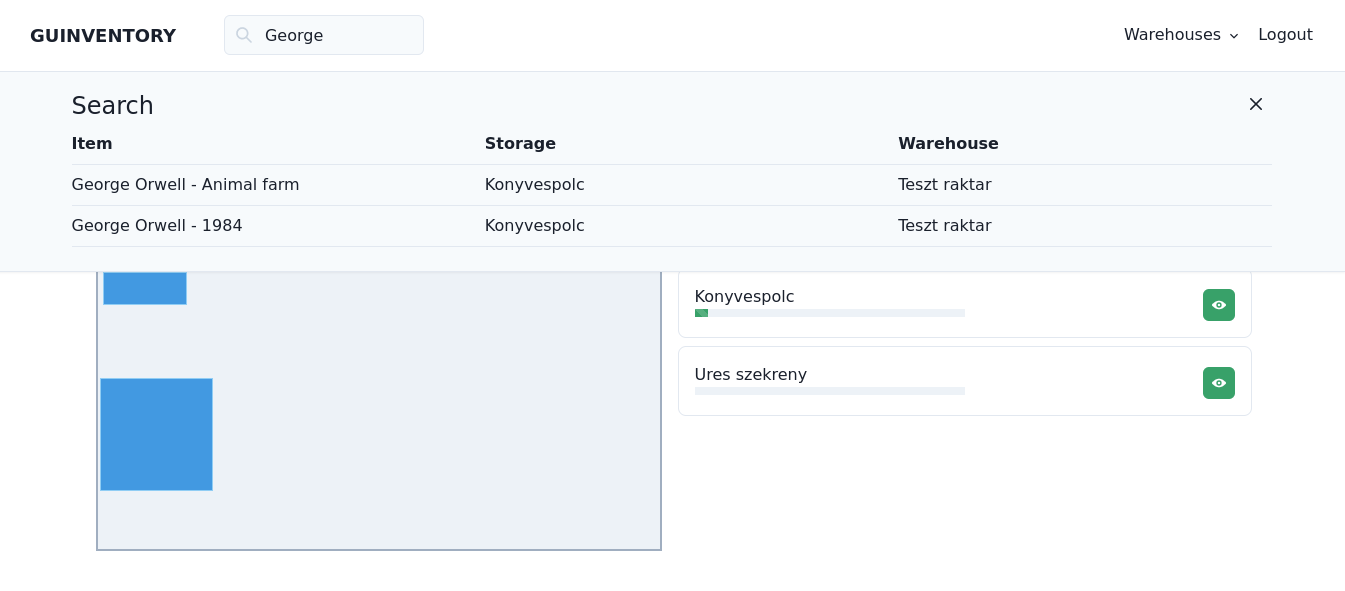
\includegraphics[width=150mm, keepaspectratio]{figures/search.png}
  \caption{Keresés}
  \label{fig:search}
\end{figure}

A keresés eredményét egy 3 oszlopos táblázatban (\refstruc{fig:search}) jelenítjük meg.
A három oszlop segítségével egyértelműen meghatározható a keresett eszköz holléte.
Lehetőségünk van a keresett eszköz raktárára, tárolójára vagy magára az eszközre navigálnunk.

A tároló nézetén (\refstruc{fig:storage}) a kurzort valamelyik eszköz fölé mozgatva megjelenítjük annak a nevét és ezen felül kiemeljük a listában is, hogy elősegítsük az azonosítást.
Természetesen ez a kiemelés másik irányba is megvalósul, tehát ha a listában választjuk ki, akkor a térképes nézeten fogjuk kiemelten látni az éppen kiválasztott eszközt.

\begin{figure}[!ht]
  \centering
  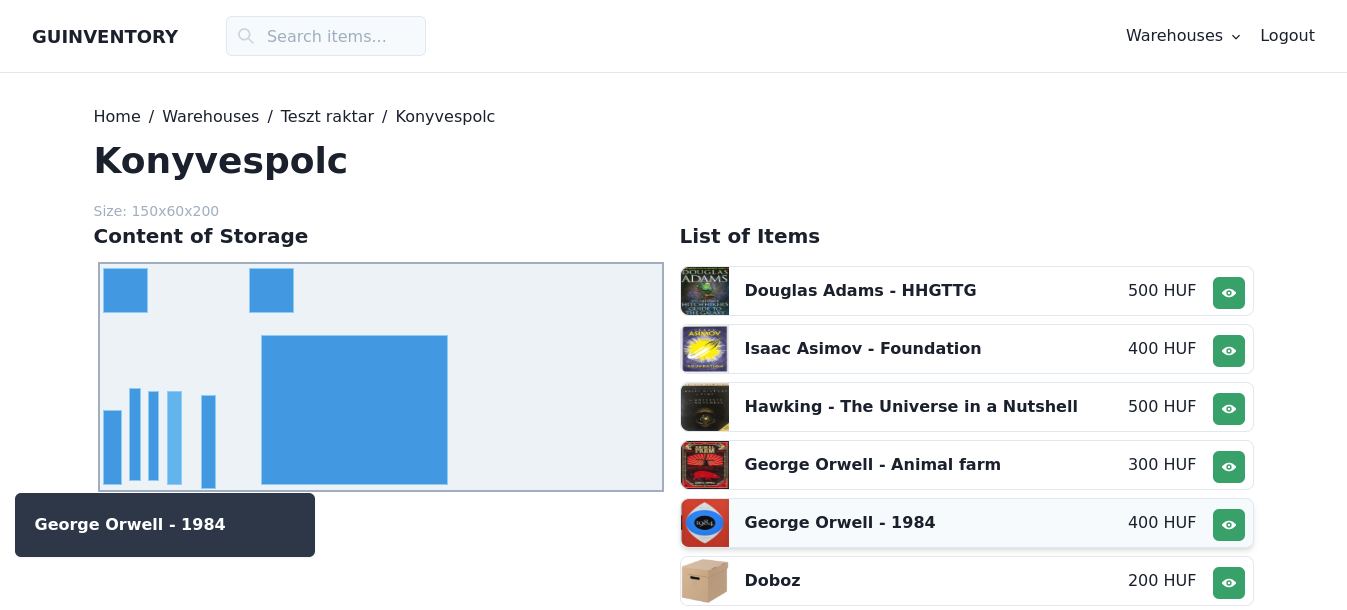
\includegraphics[width=150mm, keepaspectratio]{figures/storage.png}
  \caption{Tároló oldal}
  \label{fig:storage}
\end{figure}

A raktár nézetén belül a tárolóhoz hasonlóan kiemeléssel jelezzük az éppen kijelölt tárolót.
A tárolókról extra információként megjelenítjük az adott tároló becsült kihasználását.
A becslés a tároló méretéből és a benne tárolt eszközök méretéből számolt értékét.
Természetesen pontosan kihasználtságot nem tudunk adni, mivel a tárolókat általában nem lehet 100\%-osan kitölteni.

\begin{figure}[!ht]
  \centering
  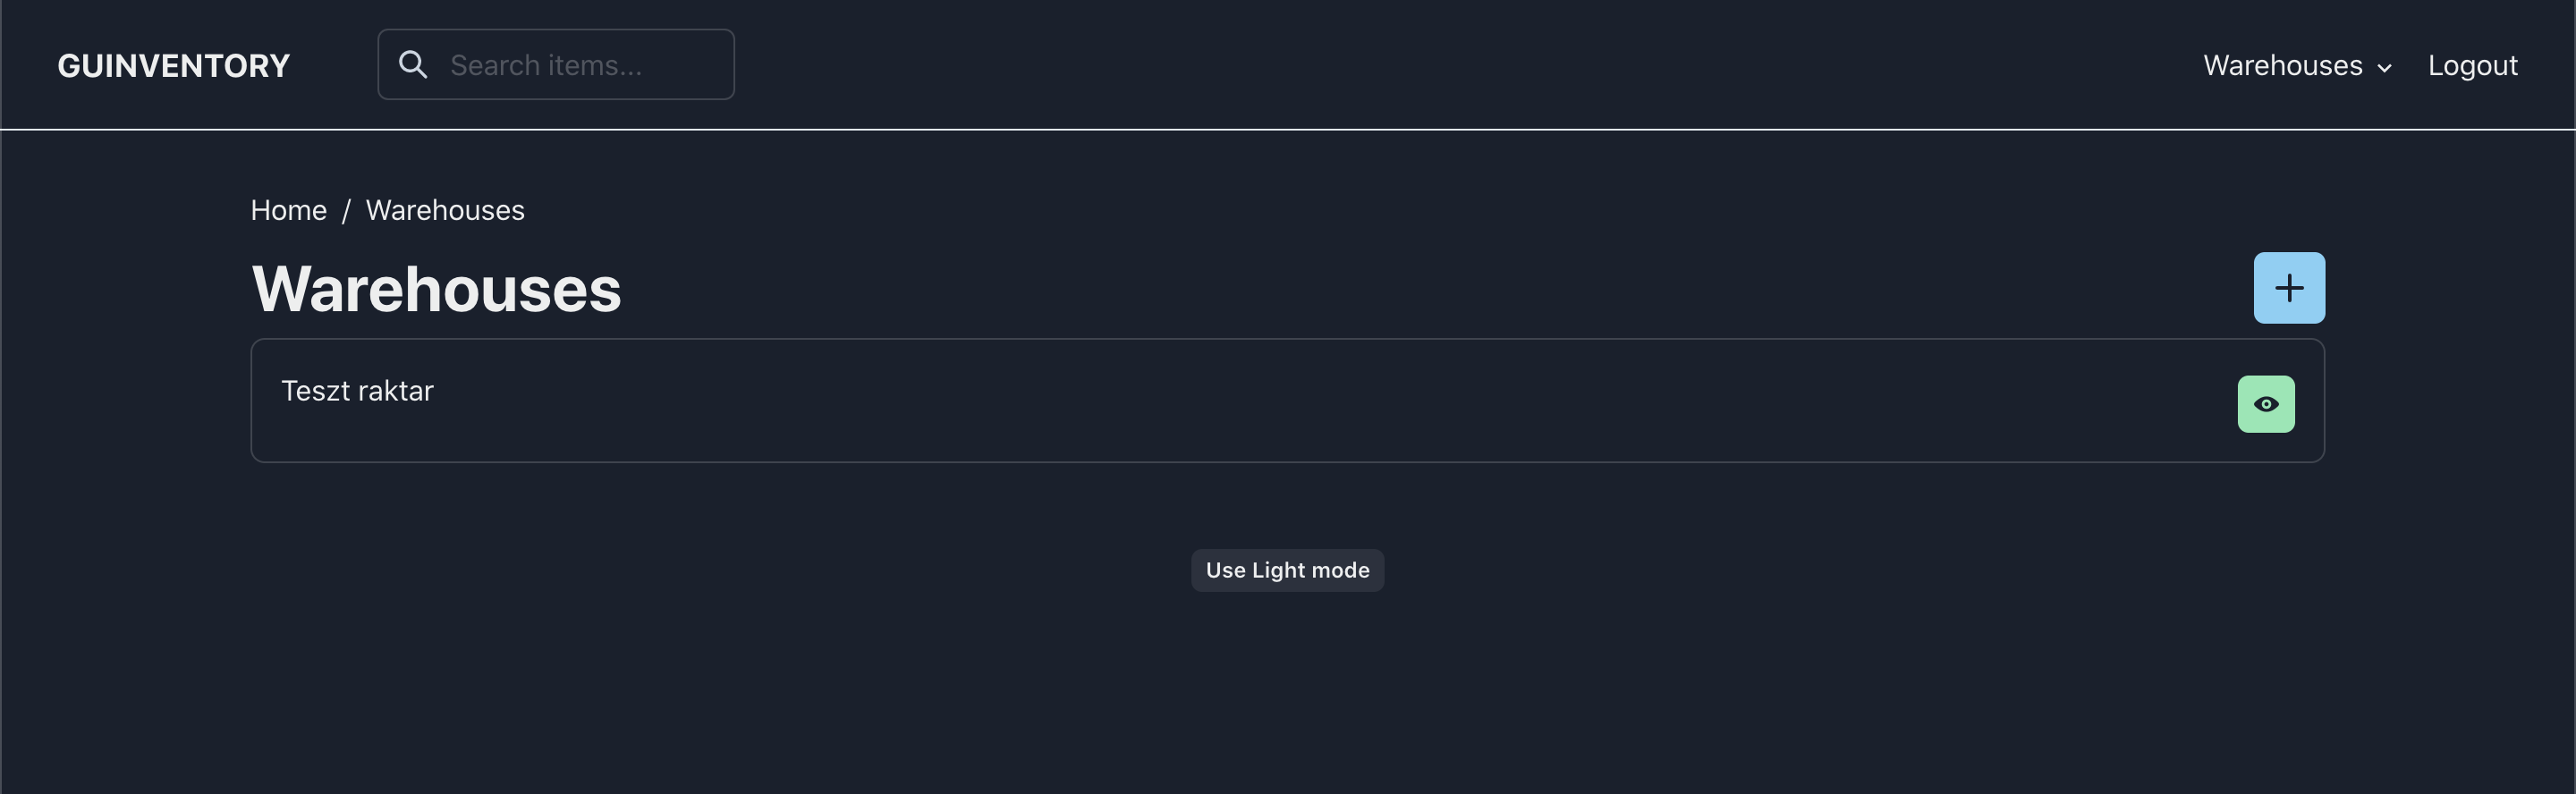
\includegraphics[width=150mm, keepaspectratio]{figures/dark_mode.png}
  \caption{Sötét téma}
  \label{fig:darkMode}
\end{figure}
A ChakraUI segítségével egyszerűen megvalósítható a sötét és világos téma is az alkalmazáshoz, valamint az e kettő közötti váltás is.
Ez jelen esetben egy sötétkék árnyalatú designt (\refstruc{fig:darkMode}) eredményezett. 
A bejelentkezett felhasználó az oldal alján található gomb segítségével válthat témát.
A választott témát az alkalmazás automatikusan elmenti a böngésző helyi tárolójába, így az oldal újbóli meglátogatásakor már a korábban kiválasztott téma lesz érvényes.


%----------------------------------------------------------------------------

% !TeX spellcheck = hu_HU
%----------------------------------------------------------------------------
\chapter{Tesztelés}
%----------------------------------------------------------------------------

Az alkalmazás működésének validációjában elengedhetetlen lépés a tesztelés.
A tesztelés ezen felül segíti a fejlesztő munkáját is, bármilyen aprónak tűnő változtatás olykor hatással lehet az alkalmazás más részeire is.
Előfordulhat, hogy már meglévő és működő funkciók válnak használhatatlanná új funkciók bevezetése közben.
Ennek a kockázatát megfelelő tesztlefedettséggel minimálisra csökkenthetjük.
%----------------------------------------------------------------------------

\section{Frontend tesztelés}

A frontend teszteléséhez úgy nevezett end–to–end teszteket készítettem.
Az E2E\footnote{end–to–end} tesztek esetén a teszt a felhasználó viselkedését szimulálja.
Egy szimulált böngészőben végzi el a tesztet és tényleges kattintás eseményt vált ki majd figyeli a renderelt képet a tesztnek megfelelő egyezést keresve.

Ezt a Jest\footnote{Jest NPM oldala \url{https://www.npmjs.com/package/jest}} és a Playwright\footnote{Playwright NPM oldala \url{https://www.npmjs.com/package/playwright}} package–ek segítségével valósítottam meg.
A tesztelés során szükség van bizonyos adatbázis adatokra, ezeket környezeti változókba helyeztem.
Jelenleg a tesztek csak lokális környezetben futnak, de a későbbi fejlesztések során így biztosítva lesz, hogy adatbázisból adatok ne kerüljenek harmadik fél kezébe.

Az alábbi példában (\refstruc{lst:e2e}) a bejelentkezés E2E tesztje látható. A bejelentkezési oldalra navigálunk, ahol kitöltjük az email és jelszó mezőket majd elküldjük a formot. A teszt rövid várakozás után ellenőrzi, hogy megtörtént–e az átirányítás és a renderelt oldal tartalmazza–e a Warehouse szöveget egy h2 HTML tag–ben.

\begin{lstlisting}[style=ES6, caption={Bejelentkezés E2E teszt},label={lst:e2e}]
it('should allow users to sign in', async () => {
  await page.goto('http://localhost:3000/auth/login')
  await page.waitForTimeout(1000)
  await page.fill('[name="email"]', process.env.TEST_USERNAME)
  await page.fill('[name="password"]', process.env.TEST_PASSWORD)
  await page.click('[type=submit]')

  await page.waitForTimeout(1000)
  await expect(page.url()).toBe('http://localhost:3000/')
  await expect(page).toHaveText('h2', 'Warehouses')
})
\end{lstlisting}

%----------------------------------------------------------------------------

\section{Backend tesztelés}
A Prisma fejlesztő csapata csupán pár hónappal ezelőtt jelentette be a 2.0–ás verziót.
A folyamatos fejlesztés ellenére is még hiányos az eszközkészlete.
Ennek köszönhetően teszteléshez sem kínál semmilyen megoldást.

A tesztelési környezet kialakításház egy SQLite adatbázist szerettem volna használni, hogy ne a fejlesztés közben használt adatbázist használjam és ne teljen túl sok időbe a tesztek futtatása.
Azonban a Prisma jelenlegi verziója nem támogatja az enumerációt SQLite adatbázis esetén.
Emiatt itt is egy PostgreSQL adatbázissal kellett dolgozom.
A tesztelés előtt egy scripttel automatikusan létrehozom a szükséges adatbázist, majd a tesztek végeztével törlöm azt, így biztosítva, hogy véletlenül se maradjon semmilyen adat az adatbázisba, ami esetleg fals eredményt váltana ki a tesztekből.

A tesztek során a GraphQL végpontot hívtam meg különböző query–kel és mutation–ökkel, majd a választ vizsgálva megbizonyosodtam a helyes működésről.


\begin{lstlisting}[style=ES6, caption=Regisztráció első teszt eset]    
test('successfully register a user', async () => {
  const data = {
    name: 'User Name',
    email: 'test.user@example.org',
    password: 'password',
  }
  const req: any = await request(config.url, register, data)

  expect(req).toHaveProperty('register')
  expect(req.register.user.email).toEqual(data.email)
})
\end{lstlisting}

% !TeX spellcheck = hu_HU
%----------------------------------------------------------------------------
\chapter{Üzemeltetés}
%----------------------------------------------------------------------------
Korábbi fejezetben írtam arról, hogy az üzemeltetést Heroku és Vercel segítségével oldottam meg.
Azonban ez az alkalmazás tényleges üzembe helyezése után nem feltétlenül a legköltséghatékonyabb módja az üzemeltetésének.
Ezért igyekeztem alternatívákat kínálni ay esetleges üzembehelyezőknek.

\section{Docker}
Az üzemeltetés megkönnyítése érdekében minden komponenshez készítettem egy-egy dockerfile-t és docker-compose file-t.

A frontendhez tartozó Docker felépítése három lépésből áll. Első lépésben a szükséges függőségeket telepítjük a yarn csomagkezelő segítségével.
Második lépésben a TypeScript kódot fordítjuk JavaScript kódra, a harmadik lépésben pedig egyszerűen elindítjuk az alkalmazást.

A három lépéses konténer készítés oka a docker cachelésénel maximális kihasználása.
Különösen nagy segítség lehet, ha ugyan azt a verziót több környezetbe is szeretnénk élesíteni.

\begin{lstlisting}[language=TeX, caption=Frontend Dockerfile]
# 1 - Install dependecies
FROM node:12-alpine AS dependencies

WORKDIR /opt/app
COPY package.json yarn.lock ./
RUN yarn install --frozen-lockfile

# 2 - Build
FROM node:12-alpine AS build

ENV NODE_ENV=production
WORKDIR /opt/app
COPY . .
COPY --from=dependencies /opt/app/node_modules ./node_modules
RUN yarn build

# 3 - Run
FROM node:12-alpine AS run

WORKDIR /opt/app
ENV NODE_ENV=production
COPY --from=build /opt/app/next.config.js ./
COPY --from=build /opt/app/public ./public
COPY --from=build /opt/app/.next ./.next
COPY --from=build /opt/app/node_modules ./node_modules
CMD ["node_modules/.bin/next", "start"]
\end{lstlisting}

A backend-hez tartozó konténer sokkalta egyszerűbb. 
A hozzá tartozó docker-compose file tartalmazza a backend és az adatbázis elindítását, valamint a közöttük lévő kapcsolat kiépítését és a Prisma Studio indítását is.

\begin{lstlisting}[language=TeX, caption=Backend docker compose]
version: '3'
services:
  server:
    build: .
    links:
      - mysql
    depends_on:
      - mysql
    ports:
      - '${SERVER_PORT}:4000'
      - '${STUDIO_PORT}:5555'
    environment:
      NODE_ENV: ${NODE_ENV}
      DATABASE_URL: ${DATABASE_URL}
      APP_SECRET: ${APP_SECRET}
    networks:
      - server-network
  mysql:
    image: mysql:5.7
    restart: always
    environment:
      MYSQL_USER: prisma
      MYSQL_PASSWORD: prisma
      MYSQL_ROOT_PASSWORD: prisma
      MYSQL_DATABASE: prisma
    networks:
      server-network:
        aliases:
          - mysql.db
    volumes:
      - db_data:/var/lib/mysql
volumes: 
  db_data:
networks:
  server-network:
\end{lstlisting}

%----------------------------------------------------------------------------

% !TeX spellcheck = hu_HU
%----------------------------------------------------------------------------
\chapter{Összefoglalás}
%----------------------------------------------------------------------------

A fejlesztés során rengeteg olyan problémát kellett megoldanom, melyekkel egyébként nem találkoztam volna.
Elmélyültem olyan technológiákban, melyek napjainkban divatosak és piaci környezetben is megállják a helyüket.
Ezeket a későbbiekben alkalmazhatom, mint tanulmányaimban, mint munkám során.
%----------------------------------------------------------------------------

\section{Tovább fejlesztési lehetőségek}
A félév során temérdek új fejlesztési lehetőség jutott eszembe, melyeket megvalósítva egy még jobb és még inkább a piaci igényeknek megfelelő alkalmazást kaphatunk.
A szakdolgozat keretein belül igyekeztem az elengedhetetlen funkciókat a lehető legjobban megvalósítani és inkább a fejlesztői eszköztár felépítését tartottam fontosnak, mint a rengeteg funkció belezsúfolását egy alkalmazásba.
Ennek köszönhetően remélhetőleg egy hosszú távon is fejleszthető és fenntartható alkalmazás született.
A félév végeztével folytatnám a munkát, hogy a lehető legtöbb piaci igényt legyen képes kiszolgálni az alkalmazásom.
%----------------------------------------------------------------------------

\subsection{Keresés}
A jelenlegi keresés egy nagyon egyszerű string összehasonlításon alapul, már egyetlen karakter elgépelése esetén sem talál egyezést.
Ennek a problémának a megoldására több lehetőség is kínálkozik, ilyen például az Elastic Search vagy a PostgreSQL–be épített full–text search.
Ezeknek az alapvető működési elve, hogy nem magában az adatbázisban keres hanem létrehoz egy index–szelt szótárat és ezt hasonlítja a keresési kifejezéshez.
Ennek köszönhetően nagy adatbázisok esetén is gyors keresés érhető el.
%----------------------------------------------------------------------------

\subsection{Egyedi tulajdonságok kezelése}
Már a félév elején felvetődött a raktárban tárolt eszközök egyedi tulajdonságainak kezelése, mint ötlet.
A tervezés során kiderült, hogy ez jóval több időt venne igénybe, mint azt az elején gondoltam, így a megvalósítását kihagytam a szakdolgozatból.

A koncepció lényege, hogy kategóriákat hozhattunk létre minden raktáron belül.
A kategóriákhoz egy név megadása után felvehetőek a tulajdonságok nevei és típusai.
Ezután az eszköz felvételekor kiválasztjuk, hogy milyen kategóriába, kategóriákba tartozik. 
Így a kategóriák révén már tudjuk azt, hogy milyen egyedi tulajdonságai lehetnek. Természetesen ehhez szükséges előredefiniált attribútum típusok létrehozására is.
%----------------------------------------------------------------------------

\subsection{3D–s térkép nézet}
Az alkalmazás már a jelenleg verziójában is tárolja a 3 dimenziós adatokat, azonban ez a megjelenítésben figyelmen kívül lett hagyva.
A későbbi fejlesztések során a jelenlegi térkép helyett egy 3 dimenziós nézet segítésével lehetőség nyílna az eszközök a valósághoz még közelebb eső állapotának tárolására egy 3 dimenziós nézet segítségével. Ennek megvalósítása azonban nagyon sok problémát vet fel, így az implementációja rengeteg időt emészthet fel.

%----------------------------------------------------------------------------



% List of Figures, Tables
%~~~~~~~~~~~~~~~~~~~~~~~~~~~~~~~~~~~~~~~~~~~~~~~~~~~~~~~~~~~~~~~~~~~~~~~~~~~~~~~~~~~~~~
\listoftables\addcontentsline{toc}{chapter}{\listtablename}


% Bibliography
%~~~~~~~~~~~~~~~~~~~~~~~~~~~~~~~~~~~~~~~~~~~~~~~~~~~~~~~~~~~~~~~~~~~~~~~~~~~~~~~~~~~~~~
\addcontentsline{toc}{chapter}{\bibname}
\bibliography{bib/mybib}


%\label{page:last}
\end{document}
